% This is a general template file for the LaTeX package SVJour3
% for Springer journals. Original by Springer Heidelberg, 2010/09/16
%
% Use it as the basis for your article. Delete % signs as needed.
%
% This template includes a few options for different layouts and
% content for various journals. Please consult a previous issue of
% your journal as needed.
%
\RequirePackage{fix-cm}
%
%\documentclass{svjour3}                     % onecolumn (standard format)
%\documentclass[smallcondensed]{svjour3}     % onecolumn (ditto)
%\documentclass[smallextended]{svjour3}       % onecolumn (second format)
\documentclass[twocolumn]{svjour3}          % twocolumn
%
\smartqed  % flush right qed marks, e.g. at end of proof
%
\usepackage{graphicx}
\usepackage{amsmath}
\usepackage{amssymb}
%
% insert here the call for the packages your document requires
%\usepackage{mathptmx}      % use Times fonts if available on your TeX system
%\usepackage{latexsym}
% etc.
%
% Jag's 
\usepackage{tabu}
\usepackage{cancel}
\usepackage{algorithm}
\usepackage{algorithmicx}
\usepackage{algpseudocode}
%\usepackage[caption=false]{subfig}
\usepackage{subcaption}
\usepackage{booktabs, mathtools}
\usepackage[dvipsnames]{xcolor}
\usepackage{url}

\captionsetup{compatibility=false}

\algdef{SE}[DOWHILE]{Do}{doWhile}{\algorithmicdo}[1]{\algorithmicwhile\ #1}%

\DeclareMathOperator{\Order}{{\mathcal O}}

% please place your own definitions here and don't use \def but
% \newcommand{}{}
\newtheorem{prop}{Proposition}
\providecommand{\HickernellFJ}{Hickernell}
\newcommand{\bm}[1]{\boldsymbol{#1}}
\newcommand{\mSigma}{\mathsf{\Sigma}}
\newcommand{\mB}{\mathsf{B}}
\newcommand{\smallocite}[1]{{\small\ocite{#1}}}
% \newcommand{\bm}[1]{\boldsymbol{#1}}
\newcommand{\dif}[1]{\text{d}{#1}}
\newcommand{\D}[1]{\text{d}{#1}}
\newcommand{\trace}[1]{\textup{trace}{#1}}

\newcommand{\naturals}{\mathbb{N}}
\newcommand{\natzero}{\mathbb{N}_0}
\newcommand{\reals}{\mathbb{R}}
\newcommand{\integers}{\mathbb{Z}}
\newcommand{\posIntegers}{\mathbb{Z}_{> 0}}
\newcommand{\complex}{\mathbb{C}}
\newcommand{\hilbert}{\mathbb{H}}
\newcommand{\Ex}{\mathbb{E}}

\newcommand{\cf}{\mathcal{F}}
\newcommand{\cx}{\mathcal{X}}
\newcommand{\tcx}{\widetilde{\cx}}
\newcommand{\rC}{\mathring{C}}
\newcommand{\rlambda}{\mathring{\lambda}}

\newcommand{\valpha}{{\bm{\alpha}}}
\newcommand{\vbeta}{{\bm{\beta}}}
\newcommand{\vDelta}{{\boldsymbol{\Delta}}}
\newcommand{\vlambda}{{\bm{\lambda}}}
\newcommand{\vphi}{{\bm{\phi}}}
\newcommand{\vpsi}{{\bm{\psi}}}
\newcommand{\vtheta}{{\bm{\theta}}}
\newcommand{\vzeta}{{\bm{\zeta}}}
\newcommand{\vthetaMLE}{\bm{\theta}_{\text{MLE}}}
\newcommand{\hvtheta}{\hat{\vtheta}}
\newcommand{\va}{\bm{a}}
\newcommand{\vA}{\bm{A}}
\newcommand{\vb}{\bm{b}}
\newcommand{\vc}{\bm{c}}
\newcommand{\vC}{\bm{C}}
\newcommand{\tvc}{\tilde{\bm{c}}}
\newcommand{\vg}{\bm{g}}
\newcommand{\vh}{\bm{h}}
\newcommand{\vf}{\bm{f}}
\newcommand{\vk}{\bm{k}}
\newcommand{\vm}{\bm{m}}
\newcommand{\vs}{\bm{s}}
\newcommand{\vt}{\bm{t}}
\newcommand{\vv}{\bm{v}}
\newcommand{\vV}{\bm{V}}
\newcommand{\vw}{\bm{w}}
\newcommand{\vW}{\bm{W}}
\newcommand{\vx}{\bm{x}}
\newcommand{\dx}{\dif{{x}}}
\newcommand{\dt}{\dif{{t}}}
\newcommand{\dvx}{\dif{\bm{x}}}
\newcommand{\dvs}{\dif{\bm{s}}}
\newcommand{\dvt}{\dif{\bm{t}}}
\newcommand{\vrho}{\bm{\rho}}
\newcommand{\hy}{\hat{y}}
\newcommand{\vy}{\bm{y}}
\newcommand{\vY}{\bm{Y}}
\newcommand{\hvy}{\hat{\vy}}
\newcommand{\vz}{\bm{z}}
\newcommand{\vZ}{\bm{Z}}
\newcommand{\dvz}{\dif{\bm{z}}}
\newcommand{\tf}{\tilde{f}}
\newcommand{\vPsi}{\boldsymbol{\Psi}}

\newcommand{\tvv}{\tilde{\vv}}
\newcommand{\tvz}{\tilde{\vz}}

\newcommand{\vCvtheta}{{C_\vtheta}}
\newcommand{\hc}{\widehat{c}}

\newcommand{\hatvy}{\hat{\bm{y}}}
\newcommand{\haty}{\hat{y}}
\newcommand{\tvy}{\tilde{\bm{y}}}
\newcommand{\ty}{\tilde{y}}
\newcommand{\vzero}{\bm{0}}
\newcommand{\vone}{\bm{1}}
\newcommand{\tvone}{\tilde{\bm{1}}}
\newcommand{\mA}{\mathsf{A}}
\newcommand{\mC}{\mathsf{C}}
\newcommand{\rmC}{\mathring{\mathsf{C}}}
\newcommand{\mCtheta}{{\mathsf{C}_{\vtheta}}}
%\newcommand{\mCthetaInv}{{\mathsf{C}^{-1}_{\vtheta}}}
%\newcommand{\mCthetaMLE}{{\mathsf{C}_{\vthetaMLE}}}
%\newcommand{\mCthetaInvMLE}{{\mathsf{C}^{-1}_{\vthetaMLE}}}
\newcommand{\mCInv}{{\mathsf{C}^{-1}}}
\newcommand{\cov}{{\textup{cov}}}
\newcommand{\var}{{\textup{var}}}


\newcommand{\tmC}{\widetilde{\mathsf{C}}}
\newcommand{\tlambda}{\tilde{\lambda}}

\newcommand{\mL}{\mathsf{L}}

\newcommand{\mLambda}{\mathsf{\Lambda}}
\newcommand{\mLambdaInv}{\mathsf{\Lambda}^{-1}}

\newcommand{\mV}{\mathsf{V}}
\newcommand{\mW}{\mathsf{W}}

\newcommand{\calN}{\mathcal{N}}
\newcommand{\me}{\mathrm{e}}

\newcommand{\tvrho}{\widetilde{\vrho}}
\newcommand{\heta}{\hat{\eta}}
\newcommand{\hmu}{\widehat{\mu}}
\newcommand{\hsigma}{\widehat{\sigma}}
\newcommand{\hnu}{\hat{\nu}}
\newcommand{\rhoCond}{\mathring{\vrho}}

\newcommand{\MLE}{\textup{MLE}}
\newcommand{\full}{\textup{full}}
\newcommand{\GCV}{\text{GCV}}
%\newcommand{\errtol}{\text{tol}}
\newcommand{\errtol}{\varepsilon}
\newcommand{\errn}{\text{err}_{n}}
\newcommand{\diag}{\text{diag}}
\newcommand{\err}{\textup{err}}
\newcommand{\code}[1]{\texttt{#1}}

\def\abs#1{\ensuremath{\left \lvert #1 \right \rvert}}
\newcommand{\norm}[2][{}]{\ensuremath{\left \lVert #2 \right \rVert}_{#1}}
\newcommand{\ip}[3][{}]{\ensuremath{\left \langle #2, #3 \right \rangle_{#1}}}

\newenvironment{nalign}{
    \begin{equation}
    \begin{aligned}
}{
    \end{aligned}
    \end{equation}
    \ignorespacesafterend
}

\providecommand{\argmin}{\operatorname*{argmin}}
\providecommand{\argmax}{\operatorname*{argmax}}
\newcommand\figref{Figure~\ref}
\newcommand\secref{Section~\ref}

\graphicspath{{./figures/}{D:/Mega/MyWriteupBackup/Sep_2ndweek_1/}}
%\graphicspath{{./figures/}}

%
% Insert the name of "your journal" with
% \journalname{myjournal}
%

\newcommand{\FJHNote}[1]{{\textcolor{blue}{FJH: #1}}}
\newcommand{\JRNote}[1]{{\textcolor{green}{JR: #1}}}


\allowdisplaybreaks[4]
\begin{document}
\setlength\abovedisplayskip{1pt}
\setlength{\belowdisplayskip}{1pt}

\title{Fast Automatic Bayesian Cubature Using Lattice Sampling
%\thanks{}
}
% Grants or other notes about the article that should go on the front
% page should be placed within the \thanks{} command in the title
% (and the %-sign in front of \thanks{} should be deleted)
%
% General acknowledgments should be placed at the end of the article.

%\subtitle{Do you have a subtitle?\\ If so, write it here}

%\titlerunning{Short form of title}        % if too long for running head

\author{R. Jagadeeswaran         \and
        Fred. J. Hickernell %etc.
}

%\authorrunning{Short form of author list} % if too long for running head

\institute{R. Jagadeeswaran \at
              Department of Applied Mathematics, \\
              Illinois Institute of Technology \\
              10 W. 32nd St., Room 208\\
              Chicago IL 60616\\
              \email{jrathin1@@iit.edu}           %  \\
%             \emph{Present address:} of F. Author  %  if needed
           \and
           Fred J. Hickernell \at
           Center for Computational Science and Department of Applied Mathematics, 
           Illinois Institute of Technology \\
           PS 106, 3105 S. Dearborn St., 
           Chicago IL 60616
           \\
           \email{hickernell@iit.edu} 
}

\date{Received: date / Accepted: date}
% The correct dates will be entered by the editor

\maketitle

\begin{abstract}
Automatic cubatures approximate multidimensional integrals to user-specified error tolerances.  For large dimensional problems, it makes sense to fix the sampling density but determine the 
sample size, $n$, automatically. Bayesian cubature postulates that the integrand is an instance of a stochastic process.  In our case, we assume a Gaussian process parameterized by a constant mean and a covariance function defined by a scale parameter and a function specifying how the integrand values at two different points in the domain are related.
These parameters are estimated from integrand values or are given non-informative priors.  This leads to credible interval for the integral.  The sample size, $n$, is chosen to make the credible interval for the Bayesian posterior error no greater than the error tolerance. 

However, the process just outlined typically requires vector-matrix operations  with a computational cost of $O(n^3)$. Our innovation is to pair low discrepancy nodes with matching kernels that lower the  computational cost to $O(n \log n)$.   This approach is demonstrated using rank-1 lattice sequences and shift-invariant kernels.  It is also implemented in the Guaranteed Automatic Integration Library (GAIL).


\keywords{Bayesian cubature \and Probabilistic numeric methods \and GAIL}
% \PACS{PACS code1 \and PACS code2 \and more}
% \subclass{MSC code1 \and MSC code2 \and more}
\end{abstract}

\section{Introduction}
\label{intro}
Cubature is the problem of inferring a numerical value for an integral, 
$ \mu := \int_{\reals^d} g(\vx) \, \dif \vx$, where $\mu$ has no closed form analytic expression. Typically, $g$ is accessible through a black-box function routine. 
Cubature is a key component of many problems in scientific computing, finance, statistical modeling, and machine learning.  \marginpar{\FJHNote{We need to make sure that all numbered equations are referenced elsewhere.}}

The integral may often be expressed as
\begin{equation}
\label{eqn:defn_mu}
\mu:= \mu(f) := \Ex[f(\boldsymbol{X})] = \int_{[0,1]^d} f(\vx)\, \dif\vx, 
\end{equation}
where $f:[0,1]^d \to \reals$ is the integrand, and $\boldsymbol{X} \sim \mathcal{U}[0,1]^d$.  The process of transforming the original integral into the form of \eqref{eqn:defn_mu}  is not addressed here.  The cubature algorithm may take the form
\begin{equation}
\label{eqn:defn_hmu}  % remove this
\hmu: = \hmu(f) := w_0 + \sum_{i=1}^{n} f(\vx_i) w_i,
\end{equation}
where the weights, $w_0$, and  $\vw = (w_i)_{i=1}^n \in \reals^n$, and the nodes, $\{\vx_i\}_{i=1}^n \subset [0,1]^d$, are chosen to make the error, $\abs{\mu - \hmu}$, small. The integration domain $[0,1]^d$ is convenient for the low discrepancy node sets that we use.  The nodes are assumed to be deterministic.

We will construct a reliable stopping criterion that determines the number of integrand values required, $n$, to ensure that the error is no greater than a user-defined error tolerance denoted $\varepsilon$, i.e., 
\begin{equation}
\label{eqn:err_crit} 
\abs{\mu - \hmu} \leq \errtol .
\end{equation}
Rather than relying on strong assumptions about the integrand, such as an upper bound on its variance or total variation, we construct a stopping criterion that is based on a credible interval arising from a Bayesian approach to the problem.  We build upon the work of Briol et al.~\cite{BriEtal18a}, Diaconis~\cite{Dia88a}, O'Hagan~\cite{OHa91a}, Ritter~\cite{Rit00a}, Rasmussen and Ghahramani~\cite{RasGha03a}, and others.  Our algorithm is an example of \emph{probabilistic numerics}.

Our primary contribution here is to demonstrate how the choice of a family of covariance kernels that match the low discrepancy sampling nodes facilitates fast computation of the cubature and the data-driven stopping criterion.  Our cubature requires $n$ function values---at a cost of $\$(f)$ each---plus $\Order(n \log(n))$ operations to check whether the error tolerance is satisfied.  The total cost of our algorithm is then $\Order(n [\$(f) + \log(n)])$.  This is significantly fewer operations than the $\Order(n^3)$ typically required for Bayesian cubature.  If function evaluation is expensive, then $\$(f)$ might be similar in magnitude to $\log(n)$.

Hickernell~\cite{Hic17a} compares different approaches to cubature error analysis depending on whether the rule is deterministic or random and whether the integrand is assumed to be deterministic or random.  Error analyis that assumes a deterministic integrand lying in a Banach space leads to an error bound that is typically impractical for deciding how large $n$ must be to satisfy \eqref{eqn:err_crit}.  The deterministic error bound includes a (semi-) norm of the integrand, which is often more complex to compute than the original integral.

Hickernell and Jim\'enez-Rugama~\cite{HicJim16a,JimHic16a} have developed stopping criteria for cubature rules based on low discrepancy nodes by tracking the decay of the discrete Fourier coefficients of the integrand.  The algorithm proposed here also relies on the discrete Fourier coefficients of the integrand, but in a different way.  Although we do not explore here automatic Bayesian cubature for relative error tolerances, the recent work by Hickernell, Jim\'enez-Rugama, and Li~\cite{HicEtal17a} suggest how this might be done.

Section \ref{sec:BC} explains the Bayesian approach to estimate the posterior cubature error and defines our automatic Bayesian cubature. Although much of this material is not new, it is included for completeness.  We end Section \ref{sec:BC}  by demonstrating why Bayesian cubature is typically quite computationally expensive.
Section \ref{sec:fast_BC}  introduces the concept of covariance kernels that match well the nodes and expedites the computations required by our automatic Bayesian cubature. 
Section \ref{sec:shift_invariant_kernel} implements this idea for shift invariant kernels and rank-1 lattice nodes.  It also describes further enhancements to the algorithm to avoid cancellation error and make it faster.  Numerical examples are provided in Section \ref{sec:NumExp} to demonstrate our new algorithm.  We conclude with a brief discussion.



\section{Bayesian cubature} \label{sec:BC}
\label{sec:1}
%Text with citations \cite{RefB} and \cite{RefJ}.

\subsection{Bayesian posterior error}
\label{sec:BayesPostErr}

Suppose that the integrand, $f$, is drawn from a Gaussian process, i.e., $f \sim \mathcal{GP}(m,s^2 C_\vtheta)$.  Specifically, $f$ has real-valued constant mean $m$ and covariance function $s^2C_\vtheta$, where $s$ is a non-negative scale factor, and $C_\vtheta: [0,1]^d \times [0,1]^d \to \mathbb{R} $ is a symmetric, positive-definite function and parameterized by $\vtheta$:
\begin{multline} \label{FJH:eq:CondPosDef}
\mC^T = \mC,  \quad \va^T \mC \va > 0 \\
\qquad \qquad  
 \text{for all } \va \ne 0, \;
  \mC = \left(  C_\vtheta(\vx_i,\vx_j)  \right)_{i,j=1}^n,\\
 n\in \mathbb{N}, \; \vx_1, \ldots, \vx_n \in [0,1]^d.
\end{multline}
The covariance function, $C$, and the Gram matrix, $\mC$ depend implicitly on $\vtheta$, but this may be omitted in the notation for simplicity's sake.

For a Gaussian process, all vectors of linear functionals of $f$ have a multivariate Gaussian distribution. Defining  $\vf  := \left( f(\vx_i)\right)_{i=1}^n$ as the multivariate normal vector of function values, it follows that 
\begin{subequations} \label{eqn:fGaussDist}
\begin{align}
\vf  & \sim \calN(m \vone, s^2 \mC), \\
\mu & \sim \calN(m, s^2 c_0), 
\\
\text{where }
c_0 &= \int_{[0,1]^{2d}} C_\vtheta(\vx,\vt) \, \dif{\vx} \, \dif{\vt}, \\
\cov(\vf, \mu) &= \left(  \int_{[0,1]^d} C(\vt,\vx_i) \, \D \vt \right)_{i=1}^n  =: \vc.
\end{align}
\end{subequations}
We need the following Lemma \ref{thrm:condDist} to derive the posterior error of our cubature.  See  \cite[(A.6), (A.11--13)]{RasWil06a} for the proof.

\begin{lemma} \label{thrm:condDist} If $\vY = (\vY_1, \vY_2)^T \sim \calN (\vm,\mC)$, where $\vY_1$ and $\vY_2$ are random vectors of arbitrary length, and 
	\begin{gather*}
	\vm = \begin{pmatrix} \vm_1 \\ \vm_2 \end{pmatrix} = \begin{pmatrix} \Ex(\vY_1) \\ \Ex(\vY_2) \end{pmatrix}, \\
	\mC = \begin{pmatrix}
	\mC_{11} & \mC_{21}^T \\ 	\mC_{21} & \mC_{22}
	\end{pmatrix} =
	\begin{pmatrix}
	\var(\vY_{1}) & \cov(\vY_{1}, \vY_2) \\ 	\cov(\vY_2,\vY_{1}) & \var(\vY_{2})
	\end{pmatrix} 
	\end{gather*}
	then 
	\begin{multline*}
	\vY_1 \vert \vY_2 \; \sim \; \calN \bigl(\vm_1 + \mC_{21}^T \mC_{22}^{-1}(\vY_2 - \vm_2), \\ \mC_{11} - \mC_{21}^T \mC_{22}^{-1} \mC_{21} \bigr).
	\end{multline*}
Moreover, the inverse of the matrix $\mC$ may be partitioned as
\begin{gather*}
\mC^{-1} = \begin{pmatrix} \mA_{11} & \mA_{21}^T \\ \mA_{21} & \mA_{22} \end{pmatrix}, \\
\mA_{11} = (\mC_{11} - \mC_{12} \mC_{22}^{-1} \mC_{21})^{-1}, \qquad 
\mA_{21} = -  \mC_{22}^{-1} \mC_{21} \mA_{11}, \\ 
\mA_{22} = \mC_{22}^{-1} + \mC_{22}^{-1} \mC_{21} \mA_{11} \mC_{21}^T \mC_{22}^{-1}.
\end{gather*}

\end{lemma}


It follows from Lemma \ref{thrm:condDist} that the \emph{conditional} distribution of the integral given observed function values, $\vf = \vy$ is also Gaussian:
\begin{multline} \label{eqn:condInteg}
\mu | (\vf = \vy) \sim \calN \bigl(m (1 - \vc^T \mC^{-1} \vone)  + \vc^T \mC^{-1} \vy, 
\\
s^2(c_0  -\vc ^T \mC^{-1} \vc) \bigr).
\end{multline}
The natural choice for  the cubature is the posterior mean of the integral, namely, 
\begin{equation}
\label{eqn:BayesCub}
\widehat{\mu}  \vert ( \vf = \vy)
= m(1 - \vone^T  \mC^{-1}\vc )
+ \vc^T \mC^{-1} \vy,
\end{equation}
which takes the form of \eqref{eqn:defn_hmu}.
Under this definition, the cubature error has zero mean and a variance depending on the choice of nodes:
\begin{equation*}
%\label{eqn_error_cond_prob}
(\mu-\hmu) | (\vf = \vy)
 \sim  \calN 
\left(
0, \;
s^2 (c_0 - \vc^T\mC^{-1}\vc) 
\right).
\end{equation*}
A credible interval for the integral is given given by 
\begin{equation}
\label{eqn_prob_confidence_interval}
\mathbb{P}_f \left[
|\mu-\hmu| \leq  2.58 s \sqrt{c_0 - \vc^T\mC^{-1}\vc } 
\right] = 99\%.
\end{equation}
Natually, the $2.58$ and $99\%$ can be replaced by other quantiles and credible levels.


\subsection{Parameter estimation}
The credible interval in \eqref{eqn_prob_confidence_interval} suggests how our automatic Bayesian cubature proceeds.  Integrand data is accumulated until the width of the credible interval is no greater than the error tolerance.  However, the credible interval still depends on the parameters $m, s$, and $\vtheta$.  These should not be assumed a priori but be inferred from the data.  This section describes three approaches.

\subsubsection{Empirical Bayes}  \label{sec:MLE}
One approach to estimate the parameters is via maximum likelihood estimation (MLE).  The log-likelihood function of the parameters given the function data $\vy$ is:
\begin{multline}
l(s,m,\vtheta | \vy)
= -\frac{1}{2} s^{-2} (\vy-m\vone)^T\mCInv(\vy-m\vone) 
\\
 - \frac{1}{2} \log(\det\, \mC) - \frac{n}{2} \log(s^2) + \text{constants.}
\end{multline}
Maximizing the log-likelihood first with respect to $m$, then with respect to $s$, and finally with respect to $\vtheta$ yields
\begin{align}
\label{eqn_m_MLE}
m_\MLE &= \frac{\vone^T \mCInv \vy }{ \vone^T \mCInv \vone} \\
\nonumber
s^2_{\MLE}  
&= \frac{1}{n} (\vy-m_{\MLE}\vone)^T\mCInv(\vy-m_{\MLE}\vone) 
\\
\label{eqn_s2_MLE}
&= 
\frac{1}{n}
\vy^T 
\left[ 
\mCInv - 
\frac{ \mCInv \vone \vone^T \mCInv }{\vone^T\mCInv \vone}
\right] \vy, \\
\nonumber
\vtheta_\MLE
&= \argmin_{\vtheta} \biggl \{
\log\left(\vy^T 
\left[ \mCInv - 
\frac{ \mCInv \vone \vone^T \mCInv }{\vone^T\mCInv \vone}
\right] \vy 
\right)  \\
\label{eqn:thetaMLE}
 & \qquad +  \frac{1}{n} \log(\det(\mC))
\biggr \}.
\end{align}
The MLE estimate of $\vtheta$ balances minimizing the covariance scale factor, $s^2_{\MLE}$, against minimizing  $\det(\mC)$. 

Under these estimates of the parameters, the cubature \eqref{eqn:BayesCub} and the credible interval \eqref{eqn_prob_confidence_interval} simplify to 
\begin{align} \label{eqn:cubMLE}
\hmu_\MLE  &= 
\left(
\frac{ (1 - \vone^T  \mCInv\vc )  \vone }{ \vone^T \mCInv \vone}   +  \vc 
\right)^T  \mCInv \vy, \\
 \label{eqn:errMLE}
\err_\MLE^2 & : = \frac{2.58^2}{n}
 \vy^T \left[ \mCInv - 
\frac{ \mCInv \vone \vone^T \mCInv }{\vone^T\mCInv \vone}
\right] \vy \\
&\qquad \qquad \times 
(c_0 - \vc^T\mC^{-1}\vc ),
\end{align}
\begin{equation}
\label{eqn_prob_CI_MLE}
\mathbb{P}_f \left[
|\mu-\hmu_\MLE| \leq \err_\MLE \right]  = 99\%.
\end{equation}
Here $c_0$, $\vc$, and $\mC$ are assumed implicitly to be based on $\vtheta = \vtheta_\MLE$.   

\subsubsection{Full Bayes}

Rather than use maximum likelihood to determine $m$ and $s$ one treat them as hyper-parameters and may a non-informative, conjugate prior, namely $\vrho_{m,s^2}(\xi, \lambda) \propto 1/\lambda$. Then the posterior density for the integral given the data using Bayes theorem is
\begin{align*}
\MoveEqLeft[1]{\rho_{\mu}(z | \vf = \vy)} \\
& \propto \int_{0}^\infty \int_{-\infty}^\infty \rho_{\mu}(z | \vf = \vy, m = \xi, s^2 = \lambda) \\
& \qquad \qquad \times  \rho_{\vf}(\vy | \xi, \lambda ) \rho_{m, s^2}(\xi, \lambda) \, \D \xi \D \lambda \\
& \propto \displaystyle \int_{0}^\infty  \frac{1}{\lambda^{(n+3)/2}} \\
& \times \int_{-\infty}^\infty  \exp \biggl( -\frac{1}{2\lambda}\biggl\{
\frac{
[z - \xi (1 - \vc^T \mC^{-1} \vone)  -  \vc^T \mC^{-1} \vy]^2}
{c_0  -\vc ^T \mC^{-1} \vc}  \\
& \qquad \qquad  + (\vy - \xi \vone)^T \mC^{-1}(\vy - \xi \vone) \biggr \} \biggr) \, \D \xi \D \lambda \\
&\qquad \qquad
\text{by \eqref{eqn:fGaussDist}, \eqref{eqn:condInteg}} \; \text{and} \; \rho_{m,s^2}(\xi,\lambda) \propto 1/\lambda \\
& \propto \displaystyle \int_{0}^\infty  \frac{1}{\lambda^{(n+3)/2}} \cdots \\ & \qquad \cdots \int_{-\infty}^\infty  \exp\left( -\frac{\alpha \xi^2 -2 \beta \xi + \gamma}{2\lambda(c_0  -\vc ^T \mC^{-1} \vc)} \right) \, \D \xi \D \lambda, \\
\intertext{where}
\alpha & = (1 - \vc^T \mC^{-1} \vone)^2 + \vone^T \mC^{-1} \vone (c_0  -\vc ^T \mC^{-1} \vc),\\
\beta & =(1 - \vc^T \mC^{-1} \vone)(z - \vc^T \mC^{-1} \vy ) \\
& \qquad \qquad  + \vone^T \mC^{-1} \vy (c_0  -\vc ^T \mC^{-1} \vc),\\
\gamma &  = (z - \vc^T \mC^{-1} \vy )^2  + \vy^T \mC^{-1} \vy (c_0  -\vc ^T \mC^{-1} \vc).
\end{align*}
In the derivation above and below, factors that are independent of $\xi$, $\lambda$, or $z$ can be discarded since we only need to preserve the proportion, however, factors that depend on $\xi$, $\lambda$, or $z$ must be kept.  
%Completing the square allows us to compute the integral with respect to $\xi$:
Completing the square $
\alpha \xi^2 -2 \beta \xi + \gamma 
= \alpha (\xi -\beta/\alpha)^2  - (\beta^2/\alpha) + \gamma,
$
allows us to evaluate the integrals with respect to $\xi$ and $\lambda$:
\begin{align*}
\MoveEqLeft{\rho_{\mu}(z | \vf = \vy)} \\
& \propto \displaystyle \int_{0}^\infty  \frac{1}{\lambda^{(n+3)/2}}  \exp\left( -\frac{  \gamma - \beta^2/\alpha}{2\lambda(c_0  -\vc ^T \mC^{-1} \vc)} \right)  \cdots \\
& \qquad \qquad \cdots \int_{-\infty}^\infty  \exp\left( -\frac{\alpha (\xi -\beta/\alpha)^2}{2\lambda(c_0  -\vc ^T \mC^{-1} \vc)} \right) \, \D \xi \D \lambda \\
& \propto \displaystyle \int_{0}^\infty  \frac{1}{\lambda^{(n+2)/2}}  \exp\left( -\frac{  \gamma - \beta^2/\alpha}{2\lambda(c_0  -\vc ^T \mC^{-1} \vc)} \right) \D \lambda \\
& \propto \left(\gamma - \frac{\beta^2}{\alpha}\right)^{-n/2} \propto \left(\alpha \gamma - \beta^2\right)^{-n/2}.
\end{align*}
Finally, we simplify the key term via straightforward calculations to the following:
\begin{equation*}
\alpha \gamma - \beta^2 \propto 1 +  \frac{(z - \hmu_{\textup{MLE}})^2}{(n-1)\widehat{\sigma}_{\textup{full}}^2}, \\
\end{equation*}
where 
\begin{multline}
\label{FJH:eq:signmaFull}
\hsigma^2_{\textup{full}} 
:= \frac{1}{n-1}
\vy^T\left[ \mC^{-1} 
- \frac{ \mC^{-1} \vone\vone^T \mC^{-1}}{\vone^T \mC^{-1} \vone}  \right]\vy
\\ 
\times  \left[\frac{(1 - \vc^T \mC^{-1} \vone)^2}{\vone^T \mC^{-1} \vone} + (c_0  -\vc ^T \mC^{-1} \vc) \right].
\end{multline}

This means that $\mu \vert (\vf = \vy )$, properly centered and scaled, has a Student's $t$-distribution with $n-1$ degrees of freedom.   The estimated integral is the same as in the empirical Bayes case, $\hmu_{\textup{full}} = \hmu_{\MLE}$, but the confidence interval is wider:
\begin{equation}
\label{eqn_prob_CI_full}
\mathbb{P}_f \left[
|\mu-\hmu_\MLE| \leq \err_{\textup{full}} \right]  = 99\%,
\end{equation}
where
\begin{equation}
\label{FJH:eq:errFull}
\err_{\textup{full}} 
:= t_{n_j-1,0.995} \hsigma_{\textup{full}} > \err_\MLE .
\end{equation}
Here $t_{n-1,0.995}$ denotes the $99.5$ percentile of a standard Student's $t$-distribution with $n-1$ degrees of freedom.

Because the shape parameter, $\vtheta$, enters the definition of the covariance kernel in a non-trivial way, the only way to treat it as a hyperparameter and assign a tractable prior would be for the prior to be discrete.  We believe in practice that choosing such a prior involves more guesswork than using the empirical Bayes estimate of $\vtheta$ in \eqref{eqn:thetaMLE} or the cross-validation approached described next.


\subsubsection{Generalized Cross-validation} \label{sec:GCV}
A third parameter optimization technique is \emph{leave-one-out cross-validation}.  Let $\widetilde{y}_i = \Ex[f(\vx_i ) | \vf_{-i} = \vy_{-i}]$, where the subscript $-i$ denotes the vector excluding the $i^{\text{th}}$ component.  This is the conditional expectation of $f(\vx_i )$ given all data but the function value at $\vx_i$.  The cross-validation criterion, which is to be minimized, is sum of squares of the difference between these conditional expectations and the observed values:
\begin{equation} \label{FJH:eq:CVA}
\textup{CV} = \sum_{i=1}^n (y_i - \widetilde{y}_i)^2.
\end{equation}

Let $\mA = \mC^{-1}$, let $\vzeta = \mA (\vy - m \vone)$, and partition $\mC$, $\mA$, and $\vzeta$ as
\begin{gather*}
\mC = \begin{pmatrix} c_{ii}  & \vC_{-i,i}^T \\  \vC_{-i,i} & \mC_{-i,-i}\end{pmatrix}, \qquad
\mA = \begin{pmatrix} a_{ii}  & \vA_{-i,i}^T \\  \vA_{-i,i} & \mA_{-i,-i}\end{pmatrix}, \\ \vzeta = \begin{pmatrix} \zeta_i   \\  \vzeta_{-i} \end{pmatrix},
\end{gather*}
where the subscript $i$ denotes the $i^{\text{th}}$ row or column, and the subscript $-i$ denotes all rows or columns except the $i^{\text{th}}$. Following this notation, Lemma \ref{thrm:condDist} implies that 
\begin{align*}
\widetilde{y}_i & = m + \vC^T_{-i,i} \mC_{-i,-i}^{-1} (\vy_{-i} -m \vone)  \\
\zeta_i  & = a_{ii}(y_i - m) + \vA_{-i,i}^T(\vy_{-i} - m \vone) \\
& = a_{ii}[(y_i - m) - \vC^T_{-i,i} \mC_{-i,-i}^{-1} (\vy_{-i} -m \vone)] \\
& = a_{ii}(y_i - \widetilde{y}_i).
\end{align*}
Thus, \eqref{FJH:eq:CVA} may be re-written as 
\begin{equation*} %\label{FJH:eq:CVB}
\textup{CV} = \sum_{i=1}^n \left(\frac{\zeta_i}{a_{ii}} \right)^2, \qquad \vzeta = \mC^{-1}(\vy - m \vone).
\end{equation*}
The generalized cross-validation criterion replaces the $i^{\text{th}}$ diagonal element of $\mA$ in the denominator by the average diagonal element of $\mA$ \cite{CraWah79a,GolHeaWah79a,Wah90}:
\begin{align} 
\nonumber
\textup{GCV} &
= \frac{\sum_{i=1}^n\zeta_i^2}{\left(\frac 1n \sum_{i=1}^n a_{ii} \right)^2} \\
\label{FJH:eq:GCV}
& = \frac{(\vy - m\vone)^T \mC^{-2} (\vy - m \vone)}{\left(\frac 1n \trace(\mC^{-1}) \right)^2}.
\end{align}

The loss function $GCV$ depends on $m$ and $\vtheta$, but not on $s$.  Minimizing the GCV  yields
\begin{equation}
m_{\textup{GCV}} = \frac{\vone^T \mC^{-2} \vy}{\vone^T \mC^{-2} \vone},\\ 
\end{equation}
\begin{multline}
\label{vthetaGCV}
\vtheta_{\textup{GCV}} = \argmin_\vtheta \left\{\log \left (  \vy^T \left[\mC^{-2} - \frac{\mC^{-2} \vone \vone^T \mC^{-2}}{\vone^T \mC^{-2} \vone}  \right] \vy \right ) \right . \\
\left . - 2 \log \left ( \trace(\mC^{-1}) \right ) \right\} .
\end{multline}
Plugging this value of $m$ into \eqref{eqn:BayesCub} yields
\begin{equation}
\label{eqn:muCV}
\widehat{\mu}_{\textup{GCV}}
= \left(\frac{(1 - \vone^T  \mC^{-1}\vc) \mC^{-1} \vone}{\vone^T \mC^{-2} \vone} + \vc \right)^T \mC^{-1} \vy.
\end{equation}

An estimate for $s$ may be obtained by noting that by Lemma \ref{thrm:condDist},
\[
\var[f(\vx_i ) | \vf_{-i} = \vy_{-i}] = s^2 a_{ii}^{-1},
\]
Thus, we may estimate $s$ using an argument similar to that used in deriving the GCV and then substituting $m_{\textup{GCV}}$ for $m$:
\begin{align}
\nonumber 
s^2 &= \var[f(\vx_i ) | \vf_{-i} = \vy_{-i}] a_{ii} \\
\nonumber 
& \approx \frac 1n \sum_{i=1}^n (y_i - \widetilde{y}_i)^2a_{ii}
 = \frac 1n \sum_{i=1}^n \frac{\zeta_i^2}{a_{ii}} \\
\nonumber 
 & \approx \frac{ \frac 1n \sum_{i=1}^n \zeta_i^2}{\frac 1n \sum_{i=1}^n a_{ii} } = \frac{(\vy - m\vone)^T \mC^{-2} (\vy - m \vone)}{ \trace(\mC^{-1}) } \\
\nonumber 
 & \approx  s^2_{\textup{GCV}} \\
 \intertext{where}
 \nonumber
 s^2_{\textup{GCV}} & : = \vy^T \left[\mC^{-2} - \frac{\mC^{-2} \vone \vone^T \mC^{-2}}{\vone^T \mC^{-2} \vone}  \right] \vy \\
 &\qquad \qquad  \qquad \qquad  \times \left[ \trace(\mC^{-1}) \right]^{-1}. \label{sGCVDef}
\end{align}

The confidence interval based on generalized cross-validation corresponds to \eqref{eqn_prob_confidence_interval} with the GCV estimates for $m$, $s$, and $\vtheta$:
\begin{gather}
\label{GCVerr}
\err_{\textup{GCV}} = 2.58 s_{\textup{GCV}}  \sqrt{c_0 - \vc^T\mC^{-1}\vc} \\
\label{GCVCI}
\mathbb{P}_f \left[
|\mu-\hmu_{\textup{GCV}}| \leq \err_{\textup{GCV}} 
\right] = 99\%.
\end{gather}

Looking back over the results of Sections  \ref{sec:MLE}--\ref{sec:GCV}, it is noted that if  the original covariance function, $C$, is replaced by $b \mC$ for some positive constant $b$, the cubature, $\hmu$, the estimates of $\vtheta$, and the credible interval widths, $\err$, all remain unchanged.  The estimates of $s^2$ are multiplied by $b^{-1}$, as would be expected. 


\subsection{The automatic Bayesian cubature algorithm}
\label{sec:bayes_cubature_algo}
The previous section presents three credible intervals, \eqref{eqn_prob_CI_MLE}, \eqref{eqn_prob_CI_full}, and \eqref{GCVCI}, for the $\mu$, the desired integral.  Each credible interval is based on different assumptions about the hyperparameters $m$, $s$, and $\vtheta$.  We stress that one must estimate these hyperparameters or assume a prior distribution on them because the credible intervals are used as stopping criteria for our cubature rule.  Since a credible intervals makes a statement about a typical function---not an outlier---one must try to ensure that the integrand is a typical draw from the assumed Gaussian process.

Our  Bayesian cubature algorithm increases the sample size until the width of the credible interval is small enough.  This is accomplished through successively doubling the sample size.  The steps are detailed in Algorithm \ref{algorithm1}.

\begin{algorithm}
\caption{Automatic Bayesian Cubature}\label{algorithm1}
  \begin{algorithmic}[1]
  	\Require a generator for the sequence
  	$\vx_1, \vx_2, \ldots$; a black-box function, $f$; an absolute error tolerance,
  	$\varepsilon>0$; the positive initial sample size, $n_0$
  	
      \State $n \gets n_0, \; n' \gets 0, \; \err = \infty$
      
      \While{$\err > \varepsilon$}

        \If{$n' > 0$}
			$n' \gets n, \ n\gets 2 n'$
		\EndIf
        \State\label{LoopStart}Generate $\{ \vx_i\}_{i=n' + 1}^{n}$ and sample $\{f(\vx_i)\}_{i=n'+1}^{n}$
        \State Compute $\vtheta$ by \eqref{eqn:thetaMLE} or \eqref{vthetaGCV}
        \State Compute $\err$, the width of the credible interval,  according to \eqref{eqn:errMLE}, \eqref{FJH:eq:errFull}, or \eqref{GCVerr}
        
        \EndWhile
        
        \State Compute $\hmu$, the approximate integral,   according to \eqref{eqn_m_MLE} or \eqref{eqn:muCV}
      \State \Return $\hmu$  and $\err$
  \end{algorithmic}
\end{algorithm}

\subsection{Example with the Matern kernel} \label{MVN_example}

To demonstrate automatic Bayesian cubature consider a Mat\'ern covariance kernel:
\begin{align}
\label{matern_kernel}
C_{\theta}(\vx, \vt) = \prod_{k=1}^d \exp(-\theta|\vx_k-\vt_k|)(1+\theta |\vx_k-\vt_k|).
\end{align}
Also, consider the integration problem of evaluating  \emph{multivariate normal probabilities}
\begin{equation}
\mu = \int_{(\va,\vb)} \frac{\exp\bigl(- \frac 12 \vt^T \mSigma^{-1} \vt \bigr)}{\sqrt{(2 \pi)^d \det(\mSigma)}} \, \dvt,
\end{equation}
where $(\va,\vb)$ is a finite, semi-infinite or infinite box in $\reals^d$.  This integral not have an analytic expression for general $\mSigma$, so cubatures are required.  

Genz \cite{Gen93} introduced a variable transformation to transform $\mu$ into an integral on the unit cube.  Let $\mSigma= \mL \mL^T$ be the Cholesky decomposition where $\mL = (l_{jk})_{j,k=1}^d$ is a lower triangular matrix.  Iteratively define
\begin{gather}
\nonumber
\alpha_1 = \Phi(a_1), \qquad \beta_1 = \Phi(b_1)
\\
\nonumber
\alpha_j(x_1,...,x_{j-1}) = 
\\
\nonumber
\Phi
\left(
\frac{1}{l_{jj}} 
\left(
a_j - \sum_{k=1}^{j-1} l_{jk} \Phi^{-1}(\alpha_k + x_k(\beta_k-\alpha_k))
\right)
\right), 
\\
\nonumber
\hspace{5cm} j=2,...,d,
\\
\nonumber
\beta_j(x_1,...,x_{j-1}) = 
\\
\nonumber
\Phi
\left(
\frac{1}{l_{jj}} 
\left(
b_j - \sum_{k=1}^{j-1} l_{jk} \Phi^{-1}(\alpha_k + x_k(\beta_k-\alpha_k))
\right)
\right), 
\\
\nonumber
\hspace{5cm} j=2,...,d,
\\
\label{fGenzdef}
f_{\text{Genz}}(\vx) = \prod_{j=1}^d [\beta_j(\vx) - \alpha_j(\vx)].
\end{gather}
where $\Phi$ is the cumulative standard normal distribution function.  Then, $\mu = \int_{[0,1]^{d-1}} f_{\text{Genz}}(\vx) \, \dvx$.

\begin{figure}
	\captionsetup[subfigure]{labelformat=empty}
	\begin{subfigure}[h]{0.48\linewidth}
		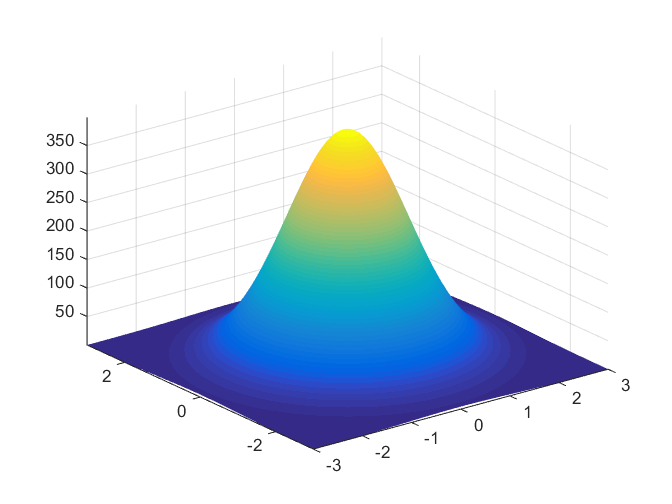
\includegraphics[width=1.1\linewidth]{Plotting_gaussian}
	\end{subfigure}
	\begin{subfigure}[h]{0.48\linewidth}
		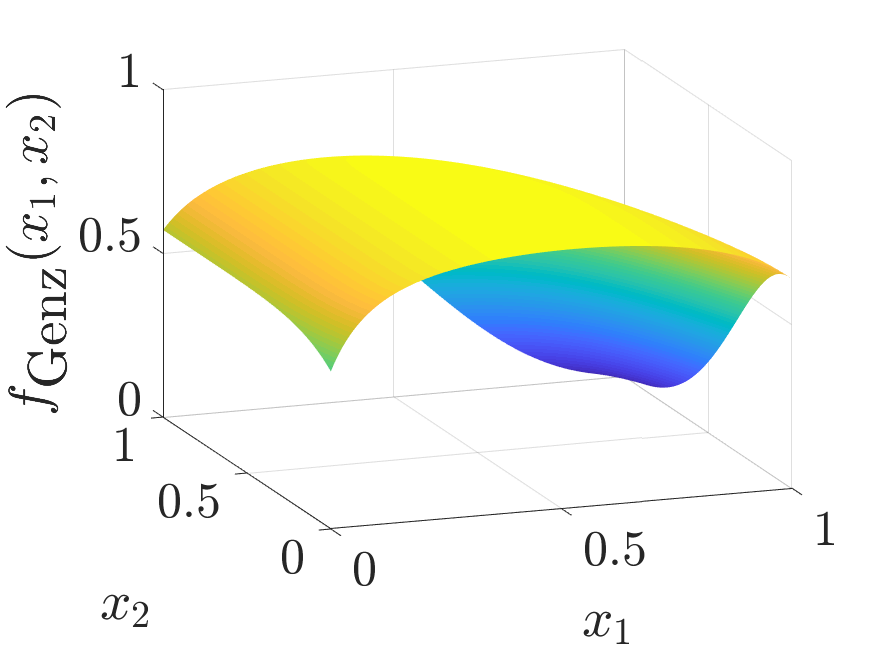
\includegraphics[width=1.1\linewidth]{GenzFunc_varTx_none}
	\end{subfigure}
	\caption{The original multivarivate Gaussian density (left) \FJHNote{Did you use your $\mL$ from below? Which dimension?}  and the transformed integrand, $f_{\text{Genz}}$ for $d=3$ (right)}
	\label{fig:MVN_Genz}
\end{figure}


We use the following parameter values in the simulation:
\begin{equation*}
\begin{array}{c|ccc}
& a  & b & L  \\
\hline
d=3
& 
\begin{pmatrix}
-6 \\ -2 \\ -2
\end{pmatrix}
& 
\begin{pmatrix}
5 \\ 2 \\ 1
\end{pmatrix} 
& 
\begin{pmatrix}
4 & 1 & 1 \\ 0 & 1 & 0.5 \\ 0 & 0 & 0.25
\end{pmatrix} 
\\
d=4
& 
\begin{pmatrix}
-6 \\ -2 \\ -2 \\ 2
\end{pmatrix}
& 
\begin{pmatrix}
5 \\ 2 \\ 1 \\2
\end{pmatrix} 
& 
\begin{pmatrix}
4 & 1 & 1 & 1\\ 0 & 1 & 0.5 & 0.5 \\ 0 & 0 & 0.25 & 0.25 \\ 0 & 0 & 0 & 0.25
\end{pmatrix} 
\end{array}
\end{equation*}


\begin{figure}
\captionsetup[subfigure]{labelformat=empty}
%\centering
\begin{subfigure}[h]{0.48\linewidth}
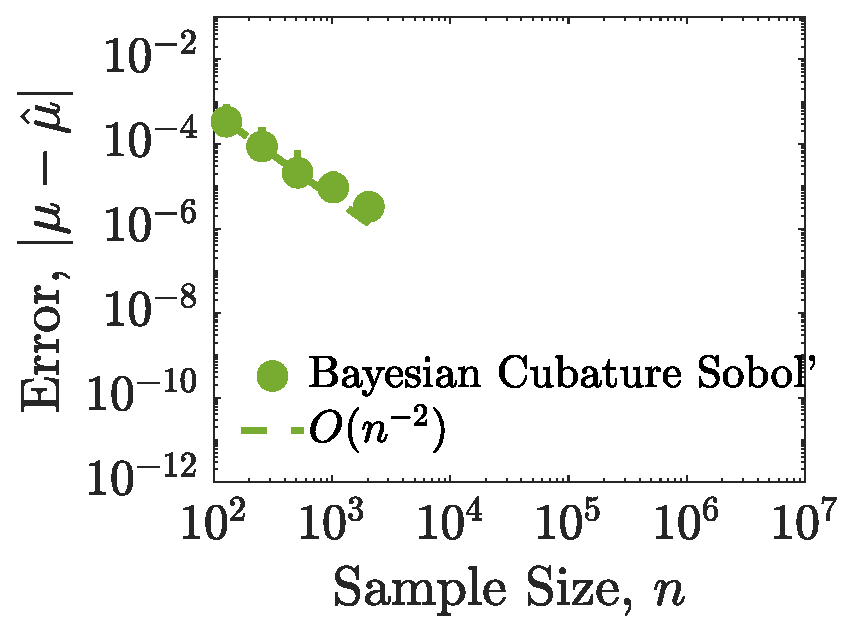
\includegraphics[width=1.1\linewidth]{MVNBayesianWtSobol}
\end{subfigure}
%\centering
\begin{subfigure}[h]{0.48\linewidth}
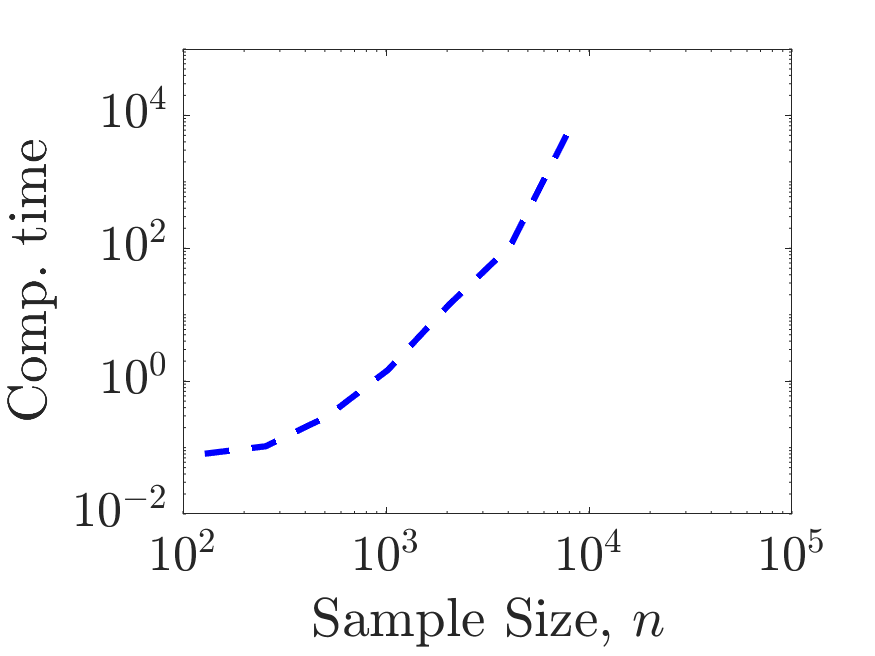
\includegraphics[width=1.1\linewidth]{MVN_bayesianCubaturecomputeTime}
\end{subfigure}
\caption{Multivariate Normal probability estimated using Matern kernel in d=2. Left: shows error redution with increase of $n$. Right: Computation time increases with increase of $n$}
\label{fig:MVN_Metern_d2b2}
\end{figure}

%with Intel i7 3630QM and 16GB RAM memory
On our test computer, it took 118 minutes to compute $\hmu_n$ with $n=2^{13}$. As shown in Figure \ref{fig:MVN_Metern_d2b2}, computation time increases rapidly with $n$. 
Especially, Maximum-likelihood-estimation of $\vtheta$ which needs the loss function, is the most time consuming of all. 
Because the loss functions need to be computed multiple times in every iteration to choose the optimal shape parameter till its minimum is found. 
Not only the complexity increases, also the kernel matrix becomes highly ill-conditioned with increasing $n$ number of data-points.
We must use alternative techniques to overcome this problem.
So, our algorithm in the current form is not straightaway usable for any practical applications.



\section{Fast Automatic Bayesian Cubature}\label{sec:fast_BC}

The generic automatic Bayesian cubature algorithm described in the previous section requires $\Order(n^3)$ operations to estimate $\vtheta$, compute the credible interval width, and compute the cubature.  There is also round-off error that can arise.  This section explains how to speed up the calculations and this round-off error.  A key is to choose kernels that match the design, $\{\vx_i\}_{i=1}^n$, so that the vector-matrix operations required by Bayesian cubature can be accomplished using fast transforms at a cost of $\Order(n \log(n))$.

\subsection{Fast transform kernel}
We make some assumptions about the relationship between the covariance kernel and the design, which will be shown to hold in Section \ref{sec:shift_invariant_kernel} for rank-1 lattices and shift-invariant kernels.  First we introduce the notation
\begin{align}
\nonumber
\mC &= \Big(C_\vtheta(\vx_i,\vx_j)\Big)_{i,j=1}^n  = (\vC_1,...,\vC_n) 
\\
\label{eqn:ftk_factor}
&= \frac 1n \mV \mLambda \mV^H , 
\quad \quad \mV^H = n \mV^{-1}, \\
\nonumber
\mV &= (\vv_1,...,\vv_n)^T = (\vV_1,...,\vV_n) \\
\nonumber
\mC^p  &= \frac 1n \mV \mLambda^{p} \mV^H, \qquad \forall p \in \integers,
\end{align}
where $\mV^H$ is the Hermitian of $\mV$.  The columns of matrix $\mV$ are eigenvectors of $\mC$, and $\mLambda$ is a diagonal matrix of eigenvalues of $\mC$.
For any $n \times n$ vector $\vb$, define the notation  $\widetilde{\vb} := \mV^H \vb$.

We make three assumptions that allow the fast computation:
\begin{subequations} \label{fastcompAssump}
	\begin{gather}
	\label{fastcompAssumpA}
	\mV \text{ may be identified analytically}, \\
	\label{fastcompAssumpB}
	\vv_1 = \vV_1 = \vone, \\
	\label{fastcompAssumpC}
	\mV^H \vb  \text{ requires only $\Order(n \log(n))$ operations } \forall \vb.
	\end{gather}
\end{subequations}
We call the transformation $\vz \mapsto \mV^H \vz$ a \emph{fast transform} and $C_\vtheta$ a \emph{fast transform kernel}.  

Under assumptions \eqref{fastcompAssump} the eigenvalues may be identified as the fast transform of the first column of $\mC$:
\begin{align}
\nonumber
\vlambda 
& = \begin{pmatrix}
\lambda_1 \\ \vdots \\ \lambda_n
\end{pmatrix} = \mLambda \vone = \mLambda \vv_1^* 
= \underbrace{\left( \frac 1n \mV^H  \mV \right) }_{\mathsf{I}} \mLambda \vv_1^* \\
&= \mV^H \left( \frac 1n \mV \mLambda \vv_1^* \right)
= \mV^H \vC_1 =  \widetilde{\vC}_1.
\label{eqn:fast_transform_to_eigvalues}
\end{align}
Also note that the fast transform of $\vone$ has a simple form
\begin{align}
\widetilde{\vone}
& = \mV^H \vone = \mV^H \vV_1 = \begin{pmatrix}n  \\ 0 \\ \vdots \\ 0 \end{pmatrix}.
\label{eqn:fast_transform_one}
\end{align}

Many of the terms that arise in the calculations in  Algorithm \ref{algorithm1} are of the form $\va^T\mC^{p}\vb$ for real $\va$ and $\vb$ and integer $p$.  These can be calculated via the transforms $\widetilde{\va} = \mV^H \va$ and $\widetilde{\vb} = \mV^H \vb$ as 
\begin{equation*}
\va^T\mC^p\vb = \frac 1n \va^T \mV \mLambda^p \mV^H \vb
= \frac 1n \widetilde{\va}^H\mLambda^p \widetilde{\vb}
= \frac 1n \sum_{i=1}^n \lambda_i^p \widetilde{a}_i^* \widetilde{b}_i, 
\end{equation*}
In particular,
\begin{align*}
\vone^T\mC^{-p}\vone & = \frac{n}{\lambda_1^p},
&
\vone^T\mC^{-p}\vy &= \frac{\widetilde{y}_1}{\lambda_1^p},
\\
\vy^T\mC^{-p} \vy &= \frac 1n \sum_{i=1}^n \frac{\abs{\widetilde{y}_i}^2}{\lambda_i^p},
&
\vc^T\mCInv \vone &= \frac{\widetilde{c}_1}{\lambda_1},\\
\vc^T\mCInv \vy &= \frac 1n \sum_{i=1}^n \frac{\widetilde{c}_i^* \widetilde{y}_i}{\lambda_i}, & 
\vc^T\mCInv \vc &= \frac 1n \sum_{i=1}^n \frac{\abs{\widetilde{c}_i}^2}{\lambda_i},
\end{align*}
where $\widetilde{\vy} = \mV^H \vy$ and 
$\widetilde{\vc} = \mV^H \vc$.  For any real $\vb$, with $\widetilde{\vb} = \mV^H\vb$, it follows that $\widetilde{b}_1$ is real since the first row of $\mV^H$ is $\vone$.

The covariance kernel used in practice also may satisfy an additional assumption:
\begin{equation} \label{addAssump}
\int_{[0,1]^d} C(\vt,\vx) \, \D \vt = 1 \qquad \forall \vx \in [0,1]^d,
\end{equation}
which implies that $c_0 = 1$ and $\vc = \vone$.  Under \eqref{addAssump}, the expressions above may be further simplified:
\begin{equation*}
\vc^T\mCInv \vone =
\vc^T\mCInv \vc = \frac{n}{\lambda_1}.
\end{equation*}


\subsection{Empirical Bayes}

Under assumptions \eqref{fastcompAssump}, the empirical Bayes parameters in \eqref{eqn_m_MLE}, \eqref{eqn_s2_MLE}, \eqref{eqn:thetaMLE} \eqref{eqn:cubMLE}, and \eqref{eqn:errMLE} can be expressed in terms of the fast transforms of the function data, the first column of the Gram matrix, and $\vc$ as follows:
\begin{align}
\nonumber
m_\MLE &=  \frac{\widetilde{y}_1}{n} = \frac 1n \sum_{i=1}^n y_i,
\\
\nonumber
s^2_\MLE 
& =
\frac{1}{n^2} 
\sum_{i=2}^n \frac{\abs{\widetilde{y}_i}^2}{\lambda_i} \\
\label{eqn_MLE_loss_func_optimized_2}\vtheta_\MLE
&= 
\argmin_{\vtheta}
\left[
\log\left(
\sum_{i=2}^n \frac{\abs{\widetilde{y}_i}^2}{\lambda_i}
\right) 
  + 
\frac{1}{n}\sum_{i=1}^n \log(\lambda_i)
\right]
\\
\hmu_\MLE  &= 
\frac{\widetilde{y}_1}{n} +
\frac 1n \sum_{i=2}^n \frac{ \widetilde{c}_i^* \widetilde{y}_i}{\lambda_i} \\
\err_\MLE  &
=
\frac{2.58}{n}\sqrt{
	\sum_{i=2}^{n} \frac{\abs{\widetilde{y}_i}^2}{\lambda_i}  
	\,
	\left( c_0 - \frac 1n \sum_{i=1}^n \frac{\abs{\widetilde{c}_i}^2}{\lambda_i} \right) 
},
\end{align}
Since all the quantities on the right hand sides can be obtained in $\Order(n \log(n))$ operations by fast transforms, the left hand sides are all computable using the asymptotic computational cost.

Under the further assumption \eqref{addAssump} it follows that 
\begin{align}
\nonumber
\hmu_\MLE  &= 
\frac{\widetilde{y}_1}{n} = \frac 1n \sum_{i=1}^n y_i,\\
\label{eq:errMLEAllAsump}
\err_\MLE  &
=
\frac{2.58}{n}\sqrt{
	\sum_{i=2}^{n} \frac{\abs{\widetilde{y}_i}^2}{\lambda_i}  
	\,
	\left( 1 -  \frac{n}{\lambda_1} \right) 
}.
\end{align}
Thus, in this  case $\hmu$ is simply the sample mean.



\subsection{Full Bayes}
For the full Bayes approach the cubature is the same as for empirical Bayes.  We also defer to empirical Bayes to estimate the parameter $\vtheta$.  The width of the confidence interval is $\err_{\textup{full}} 
:= t_{n_j-1,0.995} \hsigma_{\textup{full}}$, where $\hsigma_{\textup{full}}^2$ can also be computed swiftly under assumptions \eqref{fastcompAssump}:
\begin{multline*} %\label{FJH:eq:signmaFull}
\widehat{\sigma}^2_{\textup{full}}
=
\frac{1}{n(n-1)} \sum_{i=2}^n \frac{\abs{\widetilde{y}_i}^2}{\lambda_i}
\\
\times
\left[\frac{\lambda_1}{n}{\left(1 - \frac{\widetilde{c}_1}{\lambda_1}\right)^2} + \left(c_0  - \frac 1n \sum_{i=1}^n \frac{\abs{\widetilde{c}_i}^2}{\lambda_i}\right) \right],
\end{multline*}
Under assumption \eqref{addAssump} further simplification can be made:
\begin{equation} \label{FJH:eq:signmaFullSimple}
\widehat{\sigma}^2_{\textup{full}}
=
\frac{1}{n(n-1)} \sum_{i=2}^n \frac{\abs{\widetilde{y}_i}^2}{\lambda_i} \, \left(\frac{\lambda_1}{n}  - 1  \right),
\end{equation}
It follows that
\begin{equation} \label{FJH:eq:errFullSimple}
\err_{\textup{full}}
=
t_{n_j-1,0.995}
\sqrt{\frac{1}{n(n-1)} \sum_{i=2}^n \frac{\abs{\widetilde{y}_i}^2}{\lambda_i} \, \left(\frac{\lambda_1}{n}  - 1  \right)}.
\end{equation}


\subsection{Generalized Cross-Validation}

GCV yields a different cubature, which nevertheless can also be computed quickly using the fast transform.  Under assumptions \eqref{fastcompAssump}:
\begin{align}
\nonumber
m_{\textup{GCV}} & = m_\MLE =  \frac{\widetilde{y}_1}{n} = \frac 1n \sum_{i=1}^n y_i,\\
\nonumber 
s^2_{\textup{GCV}} & : =  \frac 1{n} \sum_{i=2}^n \frac{\abs{\widetilde{y}_i}^2}{\lambda_i^2}  \left [ \sum_{i=1}^n \frac{1}{\lambda_i} \right]^{-1}, \\
\nonumber 
\vtheta_{\textup{GCV}} 
&= \argmin_\vtheta \left[ \log \left ( \sum_{i=2}^n \frac{\abs{\widetilde{y}_i}^2}{\lambda_i^2} 
\right) \right .\\
\label{thetaGCV}
& \qquad \qquad \qquad \qquad  \left . -2\log\left( \sum_{i=1}^n \frac{1}{\lambda_i} \right)
\right], \\
\hmu_{\textup{GCV}}
&= \hmu_\MLE  = \frac{\widetilde{y}_1}{n} +
\frac 1n \sum_{i=2}^n \frac{ \widetilde{c}_i^* \widetilde{y}_i}{\lambda_i}, \\
\err_{\textup{GCV}} & =
\frac{2.58}{n^{1/2}}\left\{\sum_{i=2}^n \frac{\abs{\widetilde{y}_i}^2}{\lambda_i^2}  \left [ \sum_{i=1}^n \frac{1}{\lambda_i} \right]^{-1} \right.
\\ 
&\qquad \qquad \left . \times
\left( c_0 - \frac 1n \sum_{i=1}^n \frac{\abs{\widetilde{c}_i}^2}{\lambda_i} \right) 
\right\}^{1/2}.
\end{align}
Moreover, under further assumption \eqref{addAssump} it follows that 
\begin{align}
\label{muhatGCV-FB-MLE-Simple}
\hmu_{\textup{GCV}}
&= \hmu_\MLE = \hmu_{\textup{full}} =
\frac{\widetilde{y}_1}{n} = \frac 1n \sum_{i=1}^n y_i,\\
\nonumber
\err_{\textup{GCV}} & =
\frac{2.58}{n^{1/2}}\left\{\sum_{i=2}^n \frac{\abs{\widetilde{y}_i}^2}{\lambda_i^2}  \left [ \sum_{i=1}^n \frac{1}{\lambda_i} \right]^{-1} \right.
\\ 
&\qquad \qquad \left . \times
\left( 1 -  \frac{n}{\lambda_1} \right)  
\right\}^{1/2}. \label{errGCVSimple}
\end{align}
Thus, in this case too $\hmu$ is simply the sample mean.



\section{Integration Lattices and Shift Invariant Kernels}
\label{sec:shift_invariant_kernel}

The preceding sections lay out an automatic Bayesian cubature algorithm whose computational cost is only $\Order(n \log(n))$ if $n$ function values are used.  However, this algorithm relies on covariance kernel functions, $C$ and designs, $\{\vx_i\}_{i=1}^n$ that satisfy assumptions \eqref{fastcompAssump}.  We will also satisfy assumption \eqref{addAssump}.  To facilitate the fast transform, it is assumed in this section and the next that $n$ is power of $2$.  


\subsection{Extensible Integration Lattice Node Sets}

The design or set of nodes used is defined by a shifted extensible integration lattice node sequence, which takes the form
\begin{equation}
\vx_{i} = \vh \phi(i-1) + \vDelta \mod \vone, \qquad i \in \naturals.
\end{equation} 
Here $\vh$ is a $d$-dimensional generating vector of positive integers, $\vDelta$ is some point in $[0,1)^d$, often chosen at random, and $\{\phi(i)\}_{i=0}^n$ is the van der Corput sequence, defined by reflecting the binary digits of the integer about the decimal point, i.e., 
\begin{equation} \label{vdCDef}
\begin{array}{r|ccccccccccccc}
i & 0 & 1 & 2 & 3 & 4 &  5 & 6 & 7 & \cdots \\
i & 0_2 & 1_2 & 10_2 & 11_2 & 100_2 & 101_2 & 110_2 & 111_2  & \cdots\\
\toprule
\phi(i) & {}_2.0 &  {}_2.1 & {}_2.01 &  {}_2.11  & {}_2.001 &  {}_2.101 & {}_2.011 &  {}_2.111 & \cdots\\
\phi(i) & 0 &  0.5 &  0.25 & 0.75 &  0.125 & 0.625  &  0.375 & 0.875 & \cdots
\end{array}
\end{equation}

An example of $64$ nodes is given in Figure  \ref{latticefig}.  The even coverage of the unit cube is ensured by a well chosen generating vector.  The choice of generating vector is typically done offline by computer search.  See \cite{DicEtal14a} and \cite{HicNie03a} for more on extensible integration lattices 
\begin{figure}[htp]
	\centering
	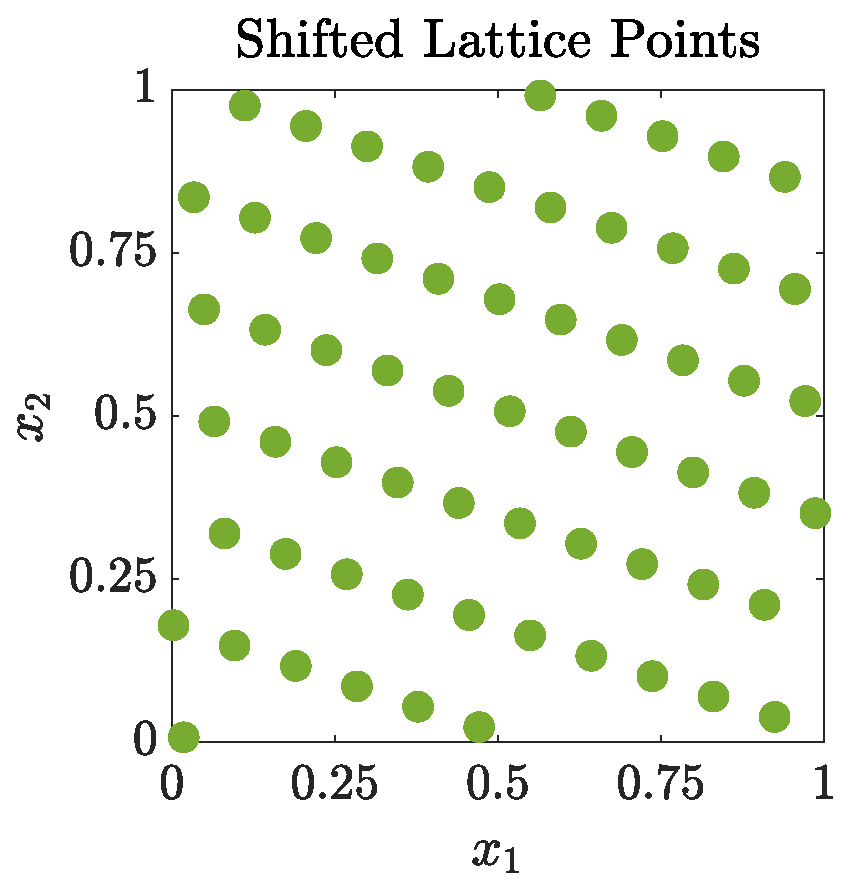
\includegraphics[height=5cm]{ShiftedLatticePoints}
	\caption{Example of a shifted integration lattice node set  in $d=2$ \label{latticefig} }
\end{figure}

\subsection{Shift Invariant Kernels}
The covariance functions $C$ that match integration lattice node sets have the form
\begin{equation} \label{eq:shInv}
C(\vt,\vx) = K(\vt - \vx \bmod \vone).
\end{equation}
This is called a \emph{shift invariant kernel} because shifting both arguments of the covariance function by the same amount leaves the value unchanged.   By a proper scaling of the kernel $K$ it follows that assumption \eqref{addAssump} is satisfied. Of course, $K$ must also be of the form that ensures that $C$ is symmetric and positive definite, as assumed in \eqref{FJH:eq:CondPosDef}. 

An family of shift invariant kernels is constructed via even degree Bernoulli polynomials:
\begin{multline}
\label{the_kernel_eqn_bernoulli}
C_\vtheta(\vt, \vx) =
\prod_{l=1}^d \biggl[
1 - (-1)^{r} \gamma B_{2r}( |{x_l-t_l}| ) \biggr], \quad  \forall \vt,\vx \in [0,1]^d, \\ \vtheta = (r,\gamma), \ r \in \naturals, \ \gamma > 0.
\end{multline}
Symmetric, positive definite kernels of this form appear in  \cite{DicEtal14a} and \cite{Hic96a}.  The Bernoulli polynomials are described in \cite[Chapter 24]{OlvEtal10a}.

Larger $r$ implies a greater degree of smoothness of the kernel.  Larger $\gamma$ implies greater fluctuations of the output with respect to the input.  Plots of $C(\cdot, 0.3)$ are given in \figref{fig:fourierkernel-dim1} for various $r$ and $\gamma$ values.

\begin{figure}
	\centering
	\includegraphics[width=0.9\linewidth]{"figures/fourier_kernel dim_1"}
	\caption[Fourier kernel]{Shift invariant kernel in 1D shifted by 0.3 to show the discontinuity }
	\label{fig:fourierkernel-dim1}
\end{figure}

\subsection{Eigenvectors}
For general shift-invariance covariance functions the Gram matrix takes the form
\begin{align}
\label{shInvKernGramMatrix}
\mC &= \bigl ( C(\vx_i, \vx_j) \bigr)_{i, j = 1}^n \\
& = \Bigl ( K(\vh(\phi(i-1) - \phi(j-1)) \bmod \vone ) \Bigr)_{i, j = 1}^n.
\end{align}

We now demonstrate that the eigenvector matrix for $\mC$ is 
\begin{equation} \label{latticeVdef}
\mV = \Bigl ( \me^{2 \pi n \sqrt{-1} \phi(i-1)\phi(j-1)} \Bigr)_{i = 1}^n.
\end{equation}
Assumption \eqref{fastcompAssumpB} follows automatically.
Now, note that the $k,j$ element of $\mV^H\mV$ is
\begin{equation*}
\sum_{i=1}^n \me^{2 \pi n \sqrt{-1} \phi(i-1)[\phi(j-1) - \phi(k-1)]}.
\end{equation*}
Noting that the sequence $\{\phi(i-1)\}_{i=1}^n$ is a re-ordering of $0, \ldots, 1-1/n$ for $n$ a power of $2$, this sum may be re-written by replacing $\phi(i-1)$ by $(i-1)/n$:
\begin{equation*}
\sum_{i=1}^n \me^{2 \pi \sqrt{-1} (i-1)[\phi(j-1) - \phi(k-1)]}.
\end{equation*}
Since $\phi(j-1) - \phi(k-1)$ is some integer multiple of $1/n$, it follows that this sum is $n \delta_{j,k}$, where $\delta$ is the Kroneker delta function.  This establishes that $\mV^H = n \mV^{-1}$ as in \eqref{eqn:ftk_factor}.

Next, let $\omega_{k, \ell}$ denote the $k,\ell$ element of $\mV^H \mC \mV$, which is given by the double sum
\begin{multline*}
\omega_{k, \ell} = \sum_{i,j=1}^n K(\vh(\phi(i-1) - \phi(j-1)) \bmod \vone ) \\
\times   \me^{-2 \pi n \sqrt{-1} \phi(k-1)\phi(i-1)}  \me^{2 \pi n \sqrt{-1} \phi(j-1)\phi(l-1)}
\end{multline*}
Noting that the sequence $\{\phi(i-1)\}_{i=1}^n$ is a re-ordering of $0, \ldots, 1-1/n$ for $n$ a power of $2$, this sum may be re-written by replacing $\phi(i-1)$ by $(i-1)/n$ and $\phi(j-1)$ by $(j-1)/n$:
\begin{multline*}
\omega_{k, \ell} = \sum_{i,j=1}^n K\left (\vh \left(\frac{i-j}{n} \right) \bmod \vone \right) \\
\times   \me^{-2 \pi \sqrt{-1} \phi(k-1)(i-1)}  \me^{2 \pi \sqrt{-1} (j-1)\phi(\ell-1)}.
\end{multline*}
This sum also remains unchanged if $i$ is replaced by $i+m$ and $j$ is replaced by $j+m$ for any integer $m$:
\begin{multline*}
\omega_{k, \ell} = \sum_{i,j=1}^n K\left (\vh \left(\frac{i-j}{n} \right) \bmod \vone \right) \\
\times   \me^{-2 \pi \sqrt{-1} \phi(k-1)(i+m-1)}  \me^{2 \pi \sqrt{-1} (j+m-1)\phi(\ell-1)} \\
=   \omega_{k, \ell}  \me^{2 \pi \sqrt{-1} m(\phi(\ell-1) - \phi(k-1))}.
\end{multline*}
For this last equality to hold for all integers $m$, we must have $k = \ell$ or $\omega_{k,\ell} = 0$.  Thus, 
\begin{align*}
\omega_{k, \ell} &= \delta_{k,\ell} \sum_{i,j=1}^n K\left (\vh \left(\frac{i-j}{n} \right) \bmod \vone \right) \\
& \qquad \qquad \qquad \qquad \times   \me^{-2 \pi \sqrt{-1} (i - j) \phi(k-1)} \\
& = n \delta_{k,\ell}  \sum_{i=1}^n K\left ( \left(\frac{i\vh}{n} \right) \bmod \vone \right)  \me^{-2 \pi \sqrt{-1} i \phi(k-1) }.
\end{align*}
This establishes $\mV^H \mC \mV$ as a diagonal matrix whose diagonal elements are $n$ times the eigenvalues, i.e., $\lambda_k = \omega_{k,k}/n$.  Furthermore, $\mV$ is the matrix of eigenvectors, which satisfies assumption \eqref{fastcompAssumpA}.

\subsection{Iterative Computation of the Fast Transform}
Assumption \eqref{fastcompAssumpA} is that computing $\mV^H \vb$ requires only $\Order(n \log(n)) $ operations.  Recall that we assume that $n$ is a power of $2$.  This can be accomplished by an iterative algorithm.  Let $\mV^{(n)}$ denote the $n \times n$ matrix $\mV$ defined in  \eqref{latticeVdef}.  We show how to compute $\mV^{(2n)H}\vb$ quickly for all $\vb \in \reals^{2n}$ assuming that $\mV^{(n)H}\vb$ can be computed quickly for all $\vb \in \reals^n$.

From the definition of the van der Corput sequence in \eqref{vdCDef} it follows that
\begin{gather} 
\label{vdCProp}
\phi(2i) = \phi(i)/2, \;  \phi(2i+1) = [\phi(i)+1]/2, \ \ \ i \in \natzero\\
\label{vdCPropB}
\phi(i+n) = \phi(i) + 1/(2n), \qquad i = 0, \ldots, n-1,
\\
\label{vdCPropC}
n \phi(i) \in \natzero, \qquad i = 0, \ldots, n-1,
\end{gather}
still assuming that $n$ is an integer power of two.
Let $\widetilde{\vb} = \mV^{(2n)H}\vb$ for some arbitrary $\vb \in \reals^{2n}$, and define
\begin{gather*}
\vb = \begin{pmatrix} b_1 \\ \vdots \\ b_{2n} \end{pmatrix}, \quad 
\vb^{(1)} = \begin{pmatrix} b_1 \\ \vdots \\ b_{n} \end{pmatrix}, \quad 
\vb^{(2)}  = \begin{pmatrix} b_{n+1} \\ \vdots \\ b_{2n} \end{pmatrix}, \\ 
\widetilde{\vb} = \begin{pmatrix} \widetilde{b}_1 \\ \vdots \\ \widetilde{b}_{2n} \end{pmatrix}, \quad 
\widetilde{\vb}^{(1)} = \begin{pmatrix} b_1 \\ b_3 \\ \vdots \\ b_{2n-1} \end{pmatrix}, \quad 
\widetilde{\vb}^{(2)}  = \begin{pmatrix} b_{2} \\  b_{4} \\ \vdots \\ b_{2n} \end{pmatrix}. 
\end{gather*}
It follows from these definitions and the definition of $\mV$ in  \eqref{latticeVdef} that
\begin{align*}
\widetilde{\vb}^{(1)} &= \left( \sum_{j=1}^{2n}  \me^{-4 \pi n \sqrt{-1} \phi(2i-2)\phi(j-1)} b_{j} \right)_{i=1}^n \\
&= \left( \sum_{j=1}^{2n}  \me^{-2 \pi n \sqrt{-1} \phi(i-1)\phi(j-1)} b_{j} \right)_{i=1}^n \quad \text{by \eqref{vdCProp}}\\
&= \left( \sum_{j=1}^{n}  \me^{-2 \pi n \sqrt{-1} \phi(i-1)\phi(j-1)} b_{j} \right)_{i=1}^n \quad \\
&\qquad \qquad +  \left( \sum_{j=1}^{n}  \me^{-2 \pi n \sqrt{-1} \phi(i-1)\phi(n+j-1)} b_{n+j} \right)_{i=1}^n \\
&= \mV^{(n)H}\vb^{(1)}  +  \biggl(  \me^{-\pi \sqrt{-1} \phi(i-1)}  \\
& \quad \times \sum_{j=1}^{n}  \me^{-2 \pi n \sqrt{-1} \phi(i-1)\phi(j-1)} b_{n+j} \biggr)_{i=1}^n \quad  \text{by \eqref{vdCPropB}}\\
&= \mV^{(n)H}\vb^{(1)} +  \left(  \me^{-\pi \sqrt{-1} \phi(i-1)} \right)_{i=1}^n \odot \bigl(\mV^{(n)H}\vb^{(2)} \bigr),
\end{align*}
where $\odot$ denotes the Hadamard (term-by-term) product.  By a similar argument, 
\begin{align*}
\widetilde{\vb}^{(2)} &= \left( \sum_{j=1}^{2n}  \me^{-4 \pi n \sqrt{-1} \phi(2i-1)\phi(j-1)} b_{j} \right)_{i=1}^n \\
&= \left( \sum_{j=1}^{2n}  \me^{-2 \pi n \sqrt{-1} [\phi(i-1)+1]\phi(j-1)} b_{j} \right)_{i=1}^n \quad \text{by \eqref{vdCProp}}\\
&= \left( \sum_{j=1}^{n}  \me^{-2 \pi n \sqrt{-1} [\phi(i-1)+1]\phi(j-1)} b_{j} \right)_{i=1}^n \quad \\
&\qquad  +  \left( \sum_{j=1}^{n}  \me^{-2 \pi n \sqrt{-1} [\phi(i-1)+1]\phi(n+j-1)} b_{n+j} \right)_{i=1}^n \\
&= \mV^{(n)H}\vb^{(1)} 
+  \left(  \me^{ -\pi \sqrt{-1} [\phi(i-1) + 1]} \right. 
\\
& \qquad \qquad \left . \times \sum_{j=1}^{n}  \me^{-2 \pi n \sqrt{-1} \phi(i-1)\phi(j-1)} b_{n+j} \right)_{i=1}^n \\
& \hspace{4cm}  \text{by \eqref{vdCPropB} and \eqref{vdCPropC}}\\
&= \mV^{(n)H}\vb^{(1)} -  \left(  \me^{-\pi \sqrt{-1} \phi(i-1)} \right)_{i=1}^n \odot \bigl(\mV^{(n)H}\vb^{(2)} \bigr).
\end{align*}

The computational cost to compute $\mV^{(2n)H}\vb$ is then twice the cost of computing $\mV^{(n)H}\vb^{(1)}$ plus $2n$ multiplications plus $2n$ additions/subtractions.  An inductive argument shows that $\mV^{(n)H}\vb$ requires only $\Order(n \log(n))$ operations.


\subsection{Overcoming Cancellation Error}
For the kernels used in our computation it may happen that $n/\lambda_1$ is close to $1$.  Thus, the term $1-n/\lambda_1$, which appears in the credible interval widths, $\err_{\MLE}$, $\err_{\textup{full}}$, and $\err_{\textup{GCV}}$, may suffer from cancellation error.  We can avoid this cancellation error by modifying how we compute the Gram matrix and its eigenvalues.

Define a new function $\rC : = C -1$, and its associated Gram matrix $\rmC = \mC - \vone \vone^T$.   Note that $\rC$ inherits the shift-invariant properties of $C$.  Since $\vone$ is the first eigenvector of $\mC$ it follows that the eigenvectors of $\rmC$ are $\rlambda_1 = \lambda_1 - n, \lambda_2, \ldots, \lambda_n$.  Moreover,
\begin{equation}
1 - \frac{n}{\lambda_1}  = \frac{\lambda_1 - n}{\lambda_1} = \frac{\rlambda_1}{\rlambda_1 +n},
\end{equation}
where now the right hand side is free of cancellation error.

We show how to compute $\rC$ without introducing round-off error.  The covariance functions that we use are of product form, namely,
\begin{equation*}
C(\vt, \vx) = \prod_{\ell=1}^d \left[1 + \rC_\ell(t_\ell,x_\ell) \right], \qquad  \rC_\ell:[0,1]^2 \to \reals.
\end{equation*}
Direct computation of $\rC (\vt,\vx) = C(\vt,\vx) -1$ introduces cancellation error if the $ \rC_\ell$ are small.  So, we employ the iteration
\begin{align*}
\rC^{(1)} &= \rC_1(t_1,x_1),  \\
\rC^{(\ell)} &  = \rC^{(\ell-1)}[1 + \rC_\ell(t_\ell,x_\ell)] + \rC_\ell(t_\ell,x_\ell), \\
& \hspace{5cm} \ell = 2, \ldots, d, \\
\rC(\vt,\vx)  & = \rC^{(d)}.
\end{align*}
In this way, the Gram matrix $\rmC$, whose $i,j$-element is $\rC(\vx_i,\vx_j)$ can be constructed with minimal round-off error.

Computing the eigenvalues of $\rmC$ via the procedure given in \eqref{eqn:fast_transform_to_eigvalues} yields $\rlambda_1 = \lambda_1 - n, \lambda_2, \ldots, \lambda_n$. The estimates of $\vtheta$ are computed in terms of the eigenvalues of $\rmC$, so \eqref{eqn_MLE_loss_func_optimized_2} and \eqref{thetaGCV} become
\begin{subequations}
\label{thetaSimple}
\begin{align}
\nonumber
\vtheta_\MLE
&= 
\argmin_{\vtheta}
\left[
\log\left(
\sum_{i=2}^n \frac{\abs{\widetilde{y}_i}^2}{\lambda_i}
\right) 
\right . \\
&
\label{thetaMLEsimple}
\qquad \qquad   \left . + 
\frac{\log(n + \rlambda_1)}{n} + \frac{1}{n}\sum_{i=2}^n \log(\lambda_i)
\right], \\
\nonumber
\vtheta_{\textup{GCV}} 
&= \argmin_\vtheta \left[ \log \left ( \sum_{i=2}^n \frac{\abs{\widetilde{y}_i}^2}{\lambda_i^2} 
\right) \right .\\
\label{thetaGCVsimple}
& \qquad \qquad  \left . -2\log\left(\frac 1{n+\rlambda_1} + \sum_{i=2}^n \frac{1}{\lambda_i} \right)
\right].
\end{align}
\end{subequations}
The widths of the credible intervals in \eqref{eq:errMLEAllAsump}, \eqref{FJH:eq:errFullSimple}, and   \eqref{errGCVSimple} become
\begin{subequations}
\label{fastStoppingCriterions}
	\begin{align}
\err_\MLE  &
=
\frac{2.58}{n}\sqrt{
	\frac{\rlambda_1}{n + \rlambda_1}
	\sum_{i=2}^{n} \frac{\abs{\widetilde{y}_i}^2}{\lambda_i}  
}, 
\\
\err_{\textup{full}} 
& = \frac{t_{n_j-1,0.995}}{n} \sqrt{
	\frac{\rlambda_1}{n-1} \sum_{i=2}^n \frac{\abs{\widetilde{y}_i}^2}{\lambda_i}
}, \\
\err_{\textup{GCV}} & =
\frac{2.58}{n^{1/2}}\sqrt{	\frac{\rlambda_1}{n + \rlambda_1} \sum_{i=2}^n \frac{\abs{\widetilde{y}_i}^2}{\lambda_i^2}  \left [ \frac{1}{n + \rlambda_1} + \sum_{i=2}^n \frac{1}{\lambda_i} \right]^{-1}} .
	\end{align}
\end{subequations}
Since $\rlambda_1 = \lambda_1 - n$ and $\lambda \sim n$ it follows $\lambda_1$ is a small value closer to 1. For significantly large $n$, credible intervals $\err_\MLE$ and $\err_\full$ are almost the same, since the Student-t distribution quantile value $t_{n_j-1,0.995}$ approaches $2.58$. 

\iffalse Whereas to compare $\err_\GCV$, need little more insight due to the term $\lambda_i^2$ in the denominator. Rewriting it:
\begin{align*}
\err_\GCV^2 & =
\frac{2.58^2}{n^2}	\frac{\rlambda_1}{n + \rlambda_1} \frac{ \sum_{i=2}^n \left( \frac{\abs{\widetilde{y}_i}^2}{\lambda_i} \frac{1}{\lambda_i} \right)}{ \frac 1n \sum_{i=1}^n \frac{1}{\lambda_i} } 
\end{align*}
If the eigenvalues are ordered with $n$ then,
\[
\frac{1}{\lambda_n} \geq \frac{1}{\lambda_{n-1}} ... \geq \frac{1}{\lambda_1} 
\]
Note that we assumed the kernel Gram matrix is positive definite, so all the eigen values are positive
\begin{align*}
\frac{ \sum_{i=2}^n \left( \frac{\abs{\widetilde{y}_i}^2}{\lambda_i} \frac{1}{\lambda_i} \right)}{ \frac 1n \sum_{i=1}^n \frac{1}{\lambda_i} } 
\leq 
\frac{ \frac{1}{\lambda_n} \sum_{i=2}^n \frac{\abs{\widetilde{y}_i}^2}{\lambda_i}  }{ \frac 1n n \frac{1}{\lambda_1} } 
\leq 
 \frac{\lambda_1}{\lambda_n} \sum_{i=2}^n  \frac{\abs{\widetilde{y}_i}^2}{\lambda_i}  
\end{align*}
Thus we can write
\begin{align*}
\err^2_\GCV \leq \frac{\lambda_1}{\lambda_n} \err^2_\MLE
\end{align*}
This shows the $\err_\GCV$ is more aggressive stopping criterion than $\err_\MLE$. If the chosen kernel is very smooth then eigen values decay very quickly with increasing $n$. 

\fi

We summarize the results of this section and the previous one as follows:
\begin{prop}
Any periodic symmetric, positive definite, shift-invariant covariance kernel of the form \eqref{eq:shInv} scaled to satisfy \eqref{addAssump}, when matched with rank-1 lattice data-sites, must satisfy assumptions \eqref{fastcompAssump}.  The \emph{fast Fourier transform} (FFT)  can be used to compute objective functions used to estimates of $\vtheta$ in \eqref{thetaSimple} and the credible interval widths \eqref{fastStoppingCriterions} in $\Order(n \log(n))$ operations.
\end{prop}


We have implemented the fast adaptive Bayesian cubature algorithm in MATLAB as part of the Guaranteed Adaptive Integration Library (GAIL) \cite{ChoEtal17b} as \allowbreak \code{cubBayesLattice\_g}. This algorithm uses the kernel defined in  \eqref{the_kernel_eqn_bernoulli} with order $r=2,4$.

\section{Numerical Experiments} \label{sec:NumExp}

\subsection{Periodizing Variable Transformations}
\label{period_var_tx}
The shift-invariant covariance kernels underlying our Bayesian cubature  assume that the integrand has a degree of periodicity, with the smoothness assumed depending on the smoothness of the kernel.  While integrands arising in practice may be smooth, they might not be periodic.  Variable transformations can be used to ensure periodicity.

Suppose that the original integral has been expressed as 
\begin{equation*}
\mu := \int_{[0,1]^d} g(\vt) \, \dif \vt
\end{equation*}
where $g$ has sufficient smoothness, but lacks periodicity.  The baker's transform,
\begin{equation} \label{eq:bakerTrans}
\vPsi: \vx \mapsto (\Psi(x_1),  \ldots, \Psi(x_d)), \quad \Psi(x)  =1 - 2 \abs{x - 1/2},
\end{equation}
allows us to write $\mu$ in the form of \eqref{eqn:defn_mu}, where $f(\vx) = g(\vPsi(\vx))$.  

A family of variable transforms take the form
\begin{subequations} \label{eq:varTrans}
\begin{equation}
\vPsi: \vx \mapsto (\Psi(x_1),  \ldots, \Psi(x_d)), \quad \Psi:[0,1] \mapsto [0,1],
\end{equation}
which allows us to write $\mu$ in the form of \eqref{eqn:defn_mu} with
\begin{equation}
f(\vx) = g(\vPsi(\vx)) \prod_{\ell = 1}^d \Psi'(x_l).
\end{equation}
\end{subequations}
If $\Psi$ is sufficiently smooth, $\lim_{x \downarrow 0}x^{-r}\Psi'(x) = \lim_{x \uparrow 1} (x-1)^{-r}\Psi'(x) = 0$ for $ r \in \natzero$, and $g \in C^{(r, \ldots, r)}[0,1]^d$, then $f$ has continuous, periodic derivatives up to order $r$ in each direction.  
Examples of this kind of transform include \cite{Lau96a}, \cite{Sid93}, \cite{Sid08a}:
\begin{align*}
C^0 &: \Psi(x) =  3 x^2 - 2 x^3, \quad   \Psi'(x) = 6x(1-x), \\
C^1 & : \Psi(x) = x^3(10-15x+6x^2),  \\
&\qquad \qquad \qquad \qquad   \Psi'(x) = 30x^2(1-x)^2 \\
\text{Sidi's } C^1 & : \Psi(x) = x - \frac{\sin(2\pi x)}{2 \pi}, \\
&\qquad \qquad \qquad \qquad   \Psi'(x) = 1 - \cos(2\pi x), \\
\text{Sidi's } C^2 & : \Psi(x) = \frac {8 - 9 \cos(\pi x) + \cos(3 \pi x)}{16} ,  \\
&\qquad \qquad \Psi'(x) = \frac {3 \pi[3 \cos(\pi x) - \cos(3 \pi x)]}{16}.
\end{align*}

Periodizing variable transforms are used for the numerical examples below.  In some cases they can speed the convergence of the Bayesian cubature. 
	



\subsection{Test Results and Observations}
\label{sec:numerical_experiments}

Three integrals were evaluated using the GAIL algorithm \code{cubBayesLattice\_g}:  a multivariate normal probability, the Keister's example, and an option pricing example.  Four different error tolerances, $\varepsilon$,  were set for each example, with the tolerances chosen depending on the difficulty of the problem.  The nodes were the randomly shifted lattice rules supplied by GAIL.  For each integral,  each tolerance, and each of our stoppinc criteria---empirical Bayes, full Bayes, and generalized cross-validation---our algorithm is run  $100$ times.  Each the execution time is plotted against $\abs{\mu - \hmu}/\varepsilon$.  We expect $\abs{\mu - \hmu}/\varepsilon$ to be no greater than one, but hope that it is not too much smaller than one, which would indicate a stopping criterion that is too conservative.


\paragraph{Multivariate Normal Probability.}

This example was already introduced in Section \ref{MVN_example}, where we used the Mat\'ern covariance kernel.  Here we apply Sidi's $C^2$  \FJHNote{????} periodization to $ f_{\textup{Genz}}$ defined in \eqref{fGenzdef}, and chose $d = 3$ and $r = \FJHNote{???}.$ The simulation results for this example function are summarized in Figures \ref{fig:mvn-guaranteed-MLE}, \ref{fig:mvn-guaranteed-FB}, and \ref{fig:mvn-guaranteed-GCV}.  In all cases the Bayesian cubature returns an approximation within the prescribed error tolerance.  

\begin{figure}
	\centering
	\includegraphics[width=0.95\linewidth]{"MVN_guaranteed_time_MLE_C2sin_d3_r4_2018-Aug-19"}
	\caption[Guaranteed:]{Multivariate normal probability example using the empirical Bayes stopping criterion.}
	\label{fig:mvn-guaranteed-MLE}
\end{figure}

\begin{figure}
	\centering
	\includegraphics[width=0.95\linewidth]{"MVN_guaranteed_time_full_C2sin_d3_r4_2018-Aug-19"}
	\caption[MVN guaranteed : FB]{Multivariate normal probability example using the full Bayes stopping criterion.}
	\label{fig:mvn-guaranteed-FB}
\end{figure}

\begin{figure}
	\centering
	\includegraphics[width=0.95\linewidth]{"MVN_guaranteed_time_GCV_C2sin_d3_r4_2018-Aug-19"}
	\caption[MVN guaranteed : GCV]{Multivariate normal probability example using the GCV stopping criterion.}
	\label{fig:mvn-guaranteed-GCV}
\end{figure}

\paragraph{Keister's Example.}

This multidimensional integral function comes from \cite{Kei96} and is inspired by a physics application:
\begin{align*}
\mu & =  \int_{\reals^d} \cos(\norm{ \vt}) \exp(-\norm{ \vt }^2) \, \dvt \\
\nonumber
&  = 
\int_{\reals^d} \cos(a\norm{ \vt}) \exp(-a\norm{ \vt }^2)  a^d \, \dvt \\
& = \int_{[0,1]^d} f_{\textup{Keister}}(\vx) \, \dvx,\\
\intertext{where }
f_\textup{Keister}(\vx) &= (2\pi)^{\frac d2} a^d \cos(a\norm{ \Phi^{-1}(\vx)}) \\
& \qquad \qquad \times \exp(-(a^2-\frac{1}{2})\norm{ \Phi^{-1}(\vx) }^2),
\end{align*}
and again $\Phi$ is the standard normal distribution.  Also, $a$ should be chosen at least as large as $1/\sqrt{2}$ to ensure that the integrand does not blow up at the boundaries of the unit cube.
%\begin{figure}
%	\captionsetup[subfigure]{labelformat=empty}
%	\begin{subfigure}[h]{0.48\linewidth}
%		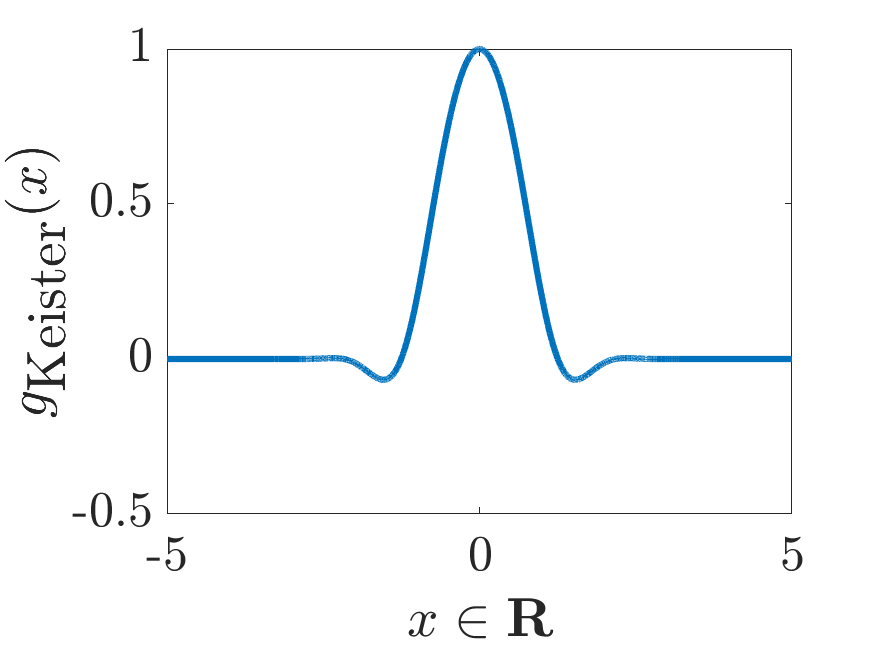
\includegraphics[width=1.1\linewidth]{Keister_wholeR_1D}
%	\end{subfigure}
%	\begin{subfigure}[h]{0.48\linewidth}
%		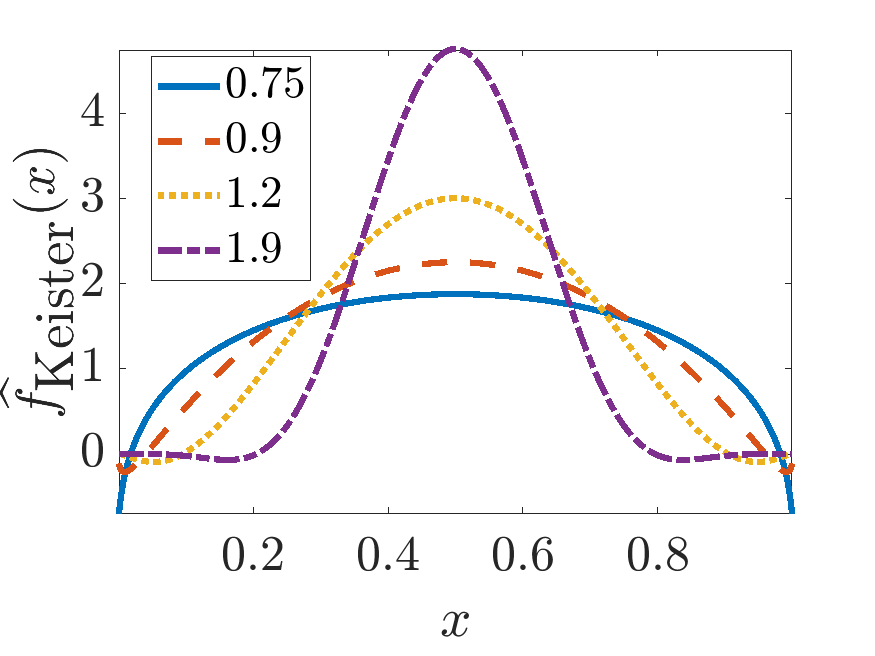
\includegraphics[width=1.1\linewidth]{Keister_cube_1D}
%	\end{subfigure}
%	\caption{Keister function in d=2 and its transformed version in $[0,1]^2$ with various values of $a$.}
%	\label{fig:keister}
%\end{figure}
The true value of $\mu$ can be calculated iteratively in terms of a quadrature as follows:  
\begin{equation*}
\mu = \frac{2 \pi^{d/2} I_c(d)}{\Gamma(d/2)}, \quad d=1,2, \ldots
\end{equation*}
where $\Gamma$ denotes the gamma function, and
\begin{align*}
I_c(1) &= \frac{\sqrt{\pi}}{2 \exp(1/4)}, 
\\
I_s(1) &= \int_{x=0}^\infty \exp(-\vx^T\vx)\sin(\vx) \, \dvx 
\\
& =  0.4244363835020225,
\\
I_c(2) &= \frac{1-I_s(1)}{2}, \qquad
I_s(2) = \frac{I_c(1)}{2}
\\
I_c(j) &= \frac{(j-2)I_c(j-2)-I_s(j-1)}{2},
\qquad j =3,4,\ldots
\\
I_s(j) &= \frac{(j-2)I_s(j-2)-I_c(j-1)}{2},
\qquad j =3,4,\ldots.
% ref: https://www.mathworks.com/help/matlab/ref/gamma.html
\end{align*}
\begin{figure}
	\centering
	\includegraphics[width=0.95\linewidth]{"Keister_guaranteed_time_MLE_C1_d4_r4_2018-Aug-19"}
	\caption[Keister guaranteed:MLE]{Keister example using the empirical Bayes stopping criterion.}
	\label{fig:keister-guaranteed-MLE}
\end{figure}
\begin{figure}
	\centering
	\includegraphics[width=0.95\linewidth]{"Keister_guaranteed_time_full_C1_d4_r4_2018-Aug-19"}
	\caption[Keister guaranteed:FB]{Keister example using the full Bayes stopping criterion.}
	\label{fig:keister-guaranteed-FB}
\end{figure}
\begin{figure}
	\centering
	\includegraphics[width=0.95\linewidth]{"Keister_guaranteed_time_GCV_C1_d4_r4_2018-Aug-19"}
	\caption[Keister guaranteed:GCV]{Keister example using the GCV stopping criterion.}
	\label{fig:keister-guaranteed-GCV}
\end{figure}

Figures \ref{fig:keister-guaranteed-MLE}, \ref{fig:keister-guaranteed-FB} and \ref{fig:keister-guaranteed-GCV} summarizes the numerical tests for this integral.  We used the $C^1$ periodization, dimension $d=4$, and $r=2$. \FJHNote{What is $a$?}
As we can see the stopping criteria is very conservative so the true errors are much smaller than user requested. \FJHNote{??} This could be attributed to the smoothness of the variable transformed ${f}_\textup{Keister}(\vt)$.

\paragraph{Option pricing}

The price of financial derivatives can often be modeled by high dimensional integrals. If the underlying asset is described in terms of a discretized geometric Brownian motion, then the the fair price of the option is:
\begin{equation*}
\mu = \int_{\reals^d} \text{payoff}(\vz) \frac{\exp(\frac 12 \vz^T\mSigma^{-1}\vz)}{\sqrt{(2\pi)^d \det(\mSigma)}} \, \dvz = \int_{[0,1]^d} f(\vx) \, \dvx,
\end{equation*} 
where {payoff($\cdot$)} defines the discounted payoff of the option,
\begin{align*}
\mSigma &= (T/d) \bigl(\min(j,k) \bigr)_{j,k=1}^d = \mL \mL^T,\\
f(\vx) &= \text{payoff} \left(\mL 
\begin{pmatrix}
\Phi^{-1}(x_1) \\ \vdots \\ \Phi^{-1}(x_d)
\end{pmatrix} \right).
\end{align*}
The Asian arithmetic mean call option has a payoff of the form
\begin{align*}
\text{payoff}(\vz) &= \max\left( \frac 1d  \sum_{j=1}^d S_j(\vz) - K, 0 \right) \me^{-r T}, \\
S_j(\vz) &= S_0 \exp\bigl((r-\sigma^2/2)jT/d + \sigma \sqrt{T/d} z_j \bigr).
\end{align*}
Here, $T$ denotes the time to maturity of the option, $d$ the number of time steps, $S_0$ the initial price of the stock, $r$ the interest rate, $\sigma$ the volatility, and $K$ the strike price.  

The Figures \ref{fig:optprice-guaranteed-MLE}, \ref{fig:optprice-guaranteed-FB} and 
\ref{fig:optprice-guaranteed-GCV} summarize the numerical results for this example using
\begin{equation*}
T = ??, \ \ d = 12, \ \ S_0 = ??, \ \ r =  ??, \ \ \sigma = ??, \ \ K = ??.
\end{equation*}
Because the integrand has a kink caused by the $\max$ function, it does not help to use a periodizing transform that is very smooth.  We choose the baker's transform and $r = 1$.

\begin{figure}
	\centering
	\includegraphics[width=0.95\linewidth]{"optPrice_guaranteed_time_MLE_Baker_d12_r2_2018-Aug-19"}
	\caption[Option pricing Guaranteed: MLE]{Option pricing using the empirical Bayes stopping criterion.}
	\label{fig:optprice-guaranteed-MLE}
\end{figure}
\begin{figure}
	\centering
	\includegraphics[width=0.95\linewidth]{"optPrice_guaranteed_time_full_Baker_d12_r2_2018-Aug-19"}
	\caption[OptPrice guaranteed : FB]{Option pricing using the full Bayes stopping criterion.}
	\label{fig:optprice-guaranteed-FB}
\end{figure}
\begin{figure}
	\centering
	\includegraphics[width=0.95\linewidth]{"optPrice_guaranteed_time_GCV_Baker_d12_r2_2018-Aug-19"}
	\caption[OptPrice guaranteed : GCV]{Option pricing using the  GCV stopping criterion.}
	\label{fig:optprice-guaranteed-GCV}
\end{figure}


As shown in Figures \ref{fig:mvn-guaranteed-MLE} to \ref{fig:optprice-guaranteed-GCV}, Bayesian cubature algorithm computes the integral within  user specified threshold most of the times except on a few occasions. This is especially the case with option pricing example due to the complexity and high dimension of the integrand. 
Also notice the algorithm finished within 10seconds of time for Keister and multivariate Normal. For the option pricing it look closer to 70seconds. This is again due to the complexity of the integrand.

Another noticeable aspect from the plots is how much estimated error differs from the true error. For option pricing example, estimated error is closer to the true error but it is not so much with Keister and multivariate Normal. This could be due to the smoothness of the integrand after the transformation. Obtaining a more accurate error estimate could be a future work.


\iffalse
\subsection{Diagnostics for the Gaussian Process Assumption}


The starting point for our Bayesian cubature is the assumption that the integrand arises from a Gaussian process. This means that the function data, $\vf$ satisfy a multivariate Gaussian distribution, as in \eqref{eqn:fGaussDist}.  The transformed data, $\vZ = ( n\mLambda)^{-\frac 12} \mV^H(\vf - m \vone)$ has zero mean and is also uncorrelated because
\begin{align*}
\cov (\vZ) 
&= \frac 1n \Ex\left[  
\mLambda^{-\frac 12} \mV^H (\vf - m \vone)
(\vf - m \vone)^T \mV \mLambda^{-\frac 12}
\right]
\\
&=
 \mLambda^{-\frac 12} \mV^H 
\Ex\left[ (\vf - m \vone)
(\vf - m \vone)^T \right] \mV \mLambda^{-\frac 12}
\\
&=
\frac{1}{n} \mLambda^{-\frac 12} \mV^H 
\frac 1n \mV \mLambda \mV^H \mV \mLambda^{-\frac 12}
 = \mathsf{I}
\end{align*}
Thus, the elements of $\vZ$ are IID standard Gaussian random variables.  

\figref{fig:mvn-normplot} and \figref{fig:keister-normplot} are normal probability plots of the $Z_i$ using empirical Bayes estimates of $m$ and $\vtheta$. \textbf{more goes here}.



\begin{figure}
	\centering
	\includegraphics[width=0.9\linewidth]{"figures/arbMean/Keister/C1sin/Keister Normplot d_2 bernoulli_2 Period_C1sin n_32768"}
	\caption{Normal plot : Keister function with arbMean assumption}
	\label{fig:keister-normplot}
\end{figure}




\begin{figure}
	\centering
	\includegraphics[width=0.9\linewidth]{"figures/arbMean/MVN/C1sin/MVN Normplot d_2 bernoulli_2 Period_C1sin n_32768"}
	\caption{Normal plot : MVN with arbMean assumption}
	\label{fig:mvn-normplot}
\end{figure}

\fi




\section{Discussion and Further Work}

We have developed a fast, automatic Bayesian cubature that estimates the integral within a user defined error tolerance.  The stopping criteria arise from assuming the integrand to be a Gaussian process.  There are three versions:  empirical Bayes, full Bayes, and generalized cross-validation.  The computational cost of the automatic Bayesian cubature can be dramatically reduced if the covariance kernel matches the nodes.  We have demonstrated one such match in practice: rank-1 lattice nodes and shift-invariant kernels.  The matrix-vector multiplications can be accomplished using the fast Fourier Transform.  Three integration problems illustrate the performance of our automatic Bayesian cubature.  

Digital sequences and digital shift and/or scramble invariant kernels have the potential of being another match that satisfies the conditions in Section \ref{sec:fast_BC}.  The fast transform would correspond to a fast Walsh transform.  For such kernels, periodicity is not assumed, however, special structure of both the sequences and the kernels are required to take advantage of integrand smoothness.

One should be able to adapt our Bayesian cubature to control variates, i.e., assuming  
\begin{equation*}
f = \mathcal{GP} \left( \beta_0 + \beta_1 g_1 + , ... , + \beta_p g_p, s^2 C \right),
\end{equation*}
for some choice of $g_1, \ldots, g_p$ whose integrals are known, and some parameters $\beta_0, \ldots, \beta_p$ in addition to the $s$ and $C$.  The efficacy of this approach has not yet been explored.




%\section{Appendix}

%\iffalse
%\subsection{Properties of Multivariate Normal Distributions}




%\fi






\iffalse

% For one-column wide figures use
\begin{figure}
% Use the relevant command to insert your figure file.
% For example, with the graphicx package use
  \includegraphics{example.eps}
% figure caption is below the figure
\caption{Please write your figure caption here}
\label{fig:1}       % Give a unique label
\end{figure}
%
% For two-column wide figures use
\begin{figure*}
% Use the relevant command to insert your figure file.
% For example, with the graphicx package use
  \includegraphics[width=0.75\textwidth]{example.eps}
% figure caption is below the figure
\caption{Please write your figure caption here}
\label{fig:2}       % Give a unique label
\end{figure*}
%
% For tables use
\begin{table}
% table caption is above the table
\caption{Please write your table caption here}
\label{tab:1}       % Give a unique label
% For LaTeX tables use
\begin{tabular}{lll}
\hline\noalign{\smallskip}
first & second & third  \\
\noalign{\smallskip}\hline\noalign{\smallskip}
number & number & number \\
number & number & number \\
\noalign{\smallskip}\hline
\end{tabular}
\end{table}

\fi



%\begin{acknowledgements}
%If you'd like to thank anyone, place your comments here
%and remove the percent signs.
%\end{acknowledgements}

% BibTeX users please use one of
%\bibliographystyle{spbasic}      % basic style, author-year citations
%\bibliographystyle{spmpsci}      % mathematics and physical sciences
%\bibliographystyle{spphys}       % APS-like style for physics
%\bibliography{}   % name your BibTeX data base
\bibliography{FJHown23,FJH23}
\bibliographystyle{spmpsci}








\iffalse
% Non-BibTeX users please use
\begin{thebibliography}{}
%
% and use \bibitem to create references. Consult the Instructions
% for authors for reference list style.
%
\bibitem{RefJ}
% Format for Journal Reference
Author, Article title, Journal, Volume, page numbers (year)
% Format for books
\bibitem{RefB}
Author, Book title, page numbers. Publisher, place (year)
% etc
\end{thebibliography}
\fi

\end{document}
% end of file template.tex